\documentclass[a4paper]{article}
%\documentclass[journal]{IEEEtran}
\usepackage{array,multirow}
\usepackage{tabu}
\usepackage{subcaption}
\usepackage{graphicx}
\usepackage{amsmath}

\begin{document}

\title{Local Directional Relation Pattern for Unconstrained and Robust Face Retrieval}

\author{Shiv Ram Dubey% <-this % stops a space
%\author{Shiv Ram Dubey, ~\IEEEmembership{Member,~IEEE}% <-this % stops a space
\thanks{
This research is funded by IIIT Sricity, India through the Faculty Seed Grant Research Fund. S.R. Dubey is associated with the Indian Institute of Information Technology Sricity, Chittoor District, AP-517646, India 
}% <-this % stops a space
}

\maketitle

\begin{abstract}
Face recognition is still a very demanding area of research. This problem becomes more challenging in unconstrained environment and in the presence of several variations like pose, illumination, expression, etc. Local descriptors are widely used for this task. The existing local descriptors are not able to utilize the wider local information to make the descriptor more discriminative. The wider local information based descriptors mainly suffer due to the increased dimensionality. In this paper, this problem is solved by encoding the relationship among directional neighbors in an efficient manner. The relationship between the center pixel and the encoded directional neighbors is utilized further to form the proposed local directional relation pattern (LDRP). The descriptor is inherently uniform illumination invariant. The multi-scale mechanism is also adapted to further boost the discriminative ability of the descriptor. The proposed descriptor is evaluated under the image retrieval framework over face databases. Very challenging databases like PaSC, LFW, PubFig, ESSEX, FERET, and AT\&T are used to test the discriminative ability and robustness of LDRP descriptor. Results are also compared with the recent state-of-the-art face descriptors such as LBP, LTP, LDP, LDN, LVP, DCP, LDGP and LGHP. Very promising performance is observed using the proposed descriptor over very appealing face databases as compared to the existing face descriptors.
\end{abstract}

%\begin{IEEEkeywords}
%Local Descriptor, Face, Unconstrained, Robust, Retrieval, %Directional Relation.
%\end{IEEEkeywords}

%\IEEEpeerreviewmaketitle

\section{Introduction}
\subsection{Motivation}
Unconstrained and robust face recognition is the current demand for the betterment of the quality life. Face is a biometric trait which can be captured very easily without making users uncomfortable and co-operative using surveillance cameras, etc. The research in this field is being done from the last two decades. Most of the early days research has been conducted in a very controlled environment, where users have given their facial images in frontal pose, under consistent lighting, without glasses or occlusion, etc. 

Some researchers also developed the face recognition approaches robust for specific geometric and photometric changes. Wright et al. used sparse representation for the face recognition \cite{wright2009}. Ding et al. proposed the pose-invariant face recognition \cite{ding2015multi}. Discriminant analysis over multi-view images are conducted for face recognition across pose \cite{kan2016multi}. Ding et al. used pose normalization for pose-invariant face recognition \cite{ding2012}. The face recognition robust to more than one effect is also investigated. Punnappurath et al. proposed the face recognition across motion blur, illumination and pose \cite{abhi2015}. The face recognition approaches are surveyed time to time by many researchers \cite{zhao2003face}, \cite{zhang2009face}, \cite{ding2016comprehensive}. 

The face recognition approaches are categorized into two major areas namely, deep learning based face recognition and descriptor based face recognition. Some recent deep learning based approaches are FaceNet \cite{facenet} and DeepFace \cite{deepface} for face recognition. The deep learning based approaches are being popular due to high performance, but at the cost of increased complexity of training in terms of the time, computing power and data size. The deep learning based approaches are also biased towards the training data.

The descriptor based face recognition approaches can be divided into learning based descriptors and handcrafted descriptors. Cao et al. learned an encoder from the training examples in unsupervised manner and applied PCA to reduce the dimension \cite{cao2010}. A family of face-image descriptors are used with learned background samples by Wolf et al. for face recognition \cite{wolf2011}. The discriminant image filters are learned with soft determined neighborhood sampling strategy \cite{lei2014}. The pixel difference vectors in local patches are mapped into low-dimensional binary vectors in an unsupervised manner to learn the binary face descriptor for Face Recognition \cite{lu2015learning}. The simultaneous local binary feature learning and encoding approach learns the binary codes and the codebook jointly for face recognition \cite{lu2015simultaneous}. The main drawback of the learning based descriptors are the dependency over the training database and vocabulary size.

The hand-designed local descriptors are very simple from design aspect. This class of descriptors have shown very promising performance in most of the computer vision problems \cite{lbpbook}. Some typical applications are local image matching \cite{iold}, image retrieval \cite{lcod},\cite{ltrp}, \cite{mdlbp}, \cite{boflbp}, texture classification \cite{lbptexture}, \cite{dlbp}, \cite{brint}, \cite{priclbp}, medical image retrieval \cite{lwp}, \cite{lbdp}, \cite{ldep}, \cite{lbdisp}, 3D face recognition \cite{tang20133d}, \cite{elaiwat2014}, etc. The main advantages of the handcrafted local descriptors are as follows: a) it is not dependent upon the database, b) it does not require very complex computing facility, and c) lower dimensional descriptors can boost the time efficiency significantly.

\subsection{Related Works}
Several face descriptors have been investigated in the last decade. Ahonen et al. applied the local binary pattern (LBP) for the face recognition \cite{lbp}. The LBP simply finds a binary code for each pixel corresponding to its neighbors. The binary code corresponding to a neighbor is 1 if the intensity value of that neighbor is greater than or equal to the intensity value of the center pixel; otherwise it is 0. The features are represented by the histogram of these binary codes. Inspired from the simplicity and success of LBP, several variants are proposed for the face recognition. Huang et al. presented a survey over facial image analysis using LBP based approaches \cite{huang2011local}. Another survey is conducted by Yang et al. over LBP based face recognition \cite{yang2013comparative}.

Some researchers tried to use the Gabor, Wavelet and Weber concepts in the framework of LBP. Zhang et al. computed the histograms of local Gabor magnitude binary pattern over different blocks of the image for representing the face images \cite{lgbphs}. The  histogram of Gabor phase pattern (HGPP) uses the orientation of Gabor wavelet and local XOR pattern for face representation \cite{hgpp}. The Fourier transform phase is quantized in local neighborhoods for blur-robust face recognition \cite{ahonen2008}. Chen et al. introduced the Weber local descriptor (WLD) which is inspired from the Weber's law \cite{wld}. The local patterns of Gabor magnitude and phase are fused by using block-based Fisher's linear discriminant for face recognition \cite{xie2010fusing}. Recently, local SVD decomposition is used with local descriptors for near infrared face retrieval \cite{svdslbp}. The drawback of such descriptors is that the time and space complexity of the transformations are too high for practical face recognition.

Instead of individual pixels, the average values of block subregions are used to compute the multi-scale block local binary pattern (MB-LBP) \cite{mblbp}. The binary concept of LBP is extended in ternary by local ternary pattern (LTP) with the help of a threshold \cite{ltp}. The local derivative pattern (LDP) computes the LBP over derivative images in four directions \cite{ldp}. Gradient edge map features are computed using a cascade of processing steps for illumination invariant frontal face representation \cite{gemf}. The relationships between gradient orientations and magnitudes like patterns of orientation difference and patterns of oriented edge magnitudes are exploited by Vu for face recognition \cite{vu2013}. Recently, Local intensity orders among two sets of local neighbors over gradient images are used to develop the local gradient order pattern for face recognition \cite{lgop}. Some researchers are trying to combine the descriptors. Recently, Lumini et al. combined the multiple descriptors like local binary pattern (LBP), histogram of oriented gradients (HOG), etc. and applied to the face recognition \cite{lumini2017}. These descriptors encode the gradient information in a local neighborhood in circular fashion but miss to utilize the directional information across different radius of the local neighborhood.

Some of the LBP variants tried to utilize the directions in order to improve it. Local directional number (LDN) pattern uses a compass mask to represent the image into different directions, then encodes it using the directional numbers and sign \cite{ldn}. Local vector pattern (LVP) uses the pairwise direction of the vector with diverse distances for each pixel to represent the face image \cite{lvp}. Jabid et al. utilized the relative magnitude's strength of edge response values in all eight directions to compute the local directional pattern for facial expression recognition \cite{jabid2010facial}. A single eight bit code for a block is used to reduce the dimensionality of the local directional pattern \cite{drldp}. Local directional gradient pattern (LDGP) uses the four directions at high order derivative space to capture the local information for recognition \cite{ldgp}. The major drawback of these approaches is the computation of directional information as a separate stage similar to pre-processing. These approaches also do not consider the directional relationship at different radius. 

Some descriptors tried to consider the wider neighborhood to increase the discriminative ability of the descriptor.
Local quantized pattern (LQP) quantizes the binary code generated from the large neighborhood with the help of a codebook to reduce the dimensionality \cite{lqp}. The LQP is computed over regional features of the image and combined using kernel fusion into a single descriptor called multiscale LQP \cite{chan2013}. In order to consider the wider neighborhood, dual cross pattern (DCP) considers the local neighbors at two radius \cite{dcp}. DCP divides the local neighborhood to reduce the dimension into two groups: first one consisting of the horizontal and vertical neighbors, whereas the second one consisting of the diagonal neighbors. DCP exploits the first derivative of Gaussian operator to encode the directional information. Very recently, the local directional ternary pattern (LDTP) has been proposed by Ryu et al. for the facial expression recognition \cite{ldtp}. It first converts the image into eight directional images using Robinson compass masks and then finds the primary and secondary directions to generate the feature vector. A very recently, the local gradient hexa pattern (LGHP) is proposed for the face recognition and retrieval \cite{lghp}. LGHP basically works by encoding the relationship of center pixel with its neighboring pixels at different distances across different derivative directions. Because LGHP uses the wider local neighborhood, its dimension is increased drastically. The major problem associated with these existing descriptors is the increased dimension while considering more local neighbors. The relationship between different neighbors in a particular direction is also not utilized by these descriptors. 

\subsection{Major Contribution}
It is pointed out from the related works that most of the descriptors use only immediate local neighbors for the feature extraction which decreases the discriminative ability of the descriptor. Some descriptors tried to utilize the wider local neighborhood, but the dimension of such descriptors is too high. The directional information in the descriptor increases the discriminative power. The existing descriptors use some filters to create the directional gradient image which increases the complexity of the descriptor.

In order to overcome the above issues of existing descriptors, this paper proposes a local directional relation pattern (LDRP). The LDRP first encodes the relationship among directional neighbors and then utilizes the encoded values with center pixel value to generate the final pattern. The major contributions are as follows:
\begin{itemize}
\item The proposed descriptor utilizes the wider local neighborhood without increasing the dimension.
\item In contrast to the existing descriptors which use derivatives to represent the directions, the LDRP descriptor uses the direction inherently. Basically, it encodes the relationship among the directional neighbors at multiple radius to transform it into a single value.
\item The proposed descriptor enriches the pattern with the relationship among local directional neighbors at multiple radius as well as the relationship between the center and transformed directional local neighboring values.
\item The relation among directional neighbors at multiple radius is computed by considering the binary relation between each pair in that direction.
\item The binary relation provides the robustness against uniform illumination while the wider local neighborhood increases the discriminative ability.
\item The proposed descriptor is experimented over six benchmarks and challenging face databases.
\end{itemize}

The rest of the paper is structured in the following manner: Section II describes the proposed descriptor; Section III illustrates the experimental setup; Section IV reports the experimental results and comparison; Section V presents the performance analysis; and finally Section V sets the concluding remarks.



\section{Proposed Descriptor}
In this section, the construction process of proposed local directional relation pattern is described in detail. The whole process is divided into several steps such as local neighborhood extraction, local directional information coding, local directional relation pattern generation, feature vector computation and multiscale adaptation.

\subsection{Local Neighborhood Extraction}
Let, $I$ is an image with dimension $x \times y$ and $I_{i,j}$ represents the intensity value for the pixel in $i^{th}$ row and $j^{th}$ column with $i \in [1,x]$ and $j \in [1,y]$. The coordinates of top and left corner is $(0,0)$ with positive x-axis downside across the rows and positive y-axis right side across the columns. The $N$ local neighbors of $I_{i,j}$ at a radius $r$ are represented by $I_{i,j}^{r}$, where $I_{i,j}^{r,k}$ is the $k^{th}$ neighbor with $k \in [1,N]$ as shown in Fig. \ref{fig:neighbors}. The coordinates of $k^{th}$ neighbor of pixel $(i,j)$ at a radius $r$ is given by $(i_k,j_k)$ defined as follows,
\begin{equation}
i_k = i + r\cos\theta_k
\end{equation}
\begin{equation}
j_k = j - r\sin\theta_k
\end{equation}
where $\theta_k$ is the angular displacement of $k^{th}$ neighbor w.r.t. first neighbor and given as follows,
\begin{equation}
\theta_k = (k-1) \times \frac{360}{N} 
\end{equation}
So, $I_{i,j}^{r,k}$ can be written as follows,
\begin{equation}
I_{i,j}^{r,k} = I_{i_k, j_k}
\end{equation}
The first neighbor is considered in the right side of the center pixel and rest of the neighbors are computed w.r.t. first neighbor in the counter-clockwise direction (see Fig. \ref{fig:neighbors}).

\begin{figure}[!t]
    \centering
    \includegraphics[width=.8\linewidth]{1.png}
    \caption{The $N$ neighbors in the local neighborhood of pixel $(i,j)$ at radius $r$. Note that the first neighbor is considered in the right side and rest neighbors are considered w.r.t. first neighbor in counter-clockwise direction.}
    \label{fig:neighbors}
\end{figure}



\subsection{Local Directional Information Coding}
In order to increase the discriminative ability of the proposed descriptor, the wider neighborhood is used in this work. The relation among local neighbors at multiple radius are utilized to encode the directional information. The $\theta_k$ represents the $k^{th}$ direction with $k\in[1,N]$. Considering the $M$ directional neighbors in $k^{th}$ direction, the binary codes are computed between each pair. The number of pairs out of $M$ neighbors are $\binom{M}{2}$. Let, the $t^{th}$ directional neighboring pair in $k^{th}$ direction is represented by ($I_{i,j}^{r_1,k}, I_{i,j}^{r_2,k}$). The index for $t^{th}$ pair can be computed from $r_1$ and $r_2$ as follows,
\begin{equation}
t = 
\begin{cases}
r_2-r_1, &\text{if $r_1=1$;}\\
r_2-r_1+\sum_{\eta=1}^{r_1-1}(m-\eta), &\text{otherwise.}
\end{cases}
\end{equation}
where $t\in[1,\binom{M}{2}]$, $r_1\in[1,M-1]$ and $r_2\in[r_1+1,M]$.

Let, $\beta_{i,j}^{k}$ denotes the local directional binary pattern for center pixel $(i,j)$ in $k^{th}$ direction. The binary code between $t^{th}$ directional neighboring pair (or between the two neighbors at radius $r_1$ and $r_2$) in $k^{th}$ direction for center pixel $(i,j)$ is generated as follows,
\begin{equation}
\beta_{i,j}^{k}(t) = 
\begin{cases}
1, &\text{if $I_{i,j}^{r_1,k} \leq I_{i,j}^{r_2,k}$;}\\
0, &\text{otherwise.}
\end{cases}
\end{equation}

\begin{figure*}[!t]
    \centering
    \includegraphics[width=.99\linewidth]{2.png}
    \caption{An illustration of the local directional relation pattern computation. (a) A local neighborhood with $N=4$ directions and $M=4$ neighbors in each direction. (b) Local direction binary bits are generated in each direction. For $M=4$, the number of binary values is $\mu=6$. (c) Local directional relation code, $\Gamma_{i,j}^{k}$, is computed in each direction for $k \in [1, 4]$ by converting $\mu=6$ binary bits into equivalent decimal. (d) The transformed center value ($\tau_{i,j}=12$) is computed from the original center pixel value ($I_{i,j}=50$) in order to match its range with local directional codes. (e) The local directional relation binary values (i.e., $\rho_{i,j}^{N,M}(k)$ for $N=4$, $M=4$ and $k \in [1,N]$) are computed for each direction. (f) Finally, the local directional relation pattern for a center pixel ($i,j$), $LDRP_{i,j}^{4,4}$, is generated from $\rho_{i,j}^{4,4}$ by converting the binary values into equivalent decimal.}
    \label{fig:example}
\end{figure*}

An example of local neighborhood with $N=4$ number of circular neighbors and $M=4$ number of directional neighbors is considered in Fig. \ref{fig:example}(a). The intensity value of the center pixel is 50 in this example. Since 4 directional neighbors at different radius is considered, $\mu=\binom{4}{2}=6$ number of binary values are generated in each direction as depicted in Fig. \ref{fig:example}(b). The local directional binary bits in $1^{st}$ direction (i.e. $0^o$) are $\beta_{i,j}^{1} = 1,1,1,0,0,1$ for the pairs (56,98),(56,75),(56,60),(98,75),(98,60),(75,60) respectively. Similarly, the local directional binary bits in $2^{nd}$ direction (i.e. $90^o$) is $\beta_{i,j}^{2} = 0,0,1,0,1,1$, in $3^{rd}$ direction (i.e. $180^o$) is $\beta_{i,j}^{3} = 1,1,1,1,1,1$, and in $4^{th}$ direction (i.e. $270^o$) is $\beta_{i,j}^{4} = 0,1,0,1,0,0$. 

For $M$ neighbors in a direction, $\mu=\binom{M}{2}$ number of binary values are generated. In order to reduce the dimension of the descriptor, it is required to code these binary values into a single value. A local directional information code ($\Gamma$) is generated in each direction from the binary values in that direction. The local directional information code, $\Gamma$, in $k^{th}$ direction for pixel $(i,j)$ is computed by the following equation, 
\begin{equation}
\Gamma_{i,j}^{k} = \sum_{\eta=1}^{\mu}(\beta_{i,j}^{k}(\eta) \times \xi(\eta))
\end{equation}
where, $\xi$ is a weight function and defined as follows,
\begin{equation}
\xi(\eta)=2^{\eta-1}.
\label{weight}
\end{equation}

The local directional relation codes in the example of Fig. \ref{fig:example}(a) are computed in Fig. \ref{fig:example}(c). The weights for $\mu=6$ directional neighbors are $\xi=1,2,4,8,16,24$. The directional relation code in $1^{st}$ direction is $\Gamma_{i,j}^{1}=1\times1+1\times2+1\times4+0\times8+0\times16+0\times64=1+2+4+0+0+0=7$. Similarly, the directional relation codes in $2^{nd}$, $3^{rd}$, and $4^{th}$ directions are $\Gamma_{i,j}^{2}=52$, $\Gamma_{i,j}^{3}=63$, and $\Gamma_{i,j}^{4}=10$ as shown in Fig. \ref{fig:example}(c).


\subsection{Local Directional Relation Pattern}
The local directional relation code is computed in the previous sub-section for a direction by encoding the relationship among the neighbors at different radius in that direction. Now, the next step is to find out the relation between center pixel and local directional relation codes. The minimum and maximum values of local directional code are dependent upon the number of directional neighbors considered (i.e. $M$). The code is generated from the $\mu = \binom{M}{2}$ number of binary values. So, the different number of decimal values that can be generated from $\mu$ binary bits is $2^{\mu}$ with a minimum value as $0$ and maximum value as $2^{\mu}-1$. Whereas, the minimum and maximum values of center pixel are $0$ and $2^{B}-1$ respectively, where $B$ is the bit-depth of the image. Note that, the bit-depth ($B$) of the images is 8 in the databases used in this paper. A clear mismatch can be observed between the range of center pixel and local directional relation code. Thus, a transformation is required over either the center pixel or the local directional relation codes to match both the ranges. Due to efficiency reason, the center pixel is transformed into the range of local directional relation codes as follows,
\begin{equation}
\tau_{i,j} = \Upsilon (I_{i,j} \times \frac{2^{\mu}-1}{2^{B}-1}).
\end{equation}
where, $\tau_{i,j}$ is the transformed version of $I_{i,j}$, $\Upsilon(\eta)$ is a function to round $\eta$ to the closest integer value.
The transformed value of center pixel in Fig. \ref{fig:example}(d) for $\mu=6$ and $B=8$ is computed as $\tau_{i,j}=\Upsilon(50 \times \frac{2^6-1}{2^8-1})=12$.

Let, $\rho$ is a binary pattern representing the relationship between center and directional relation code having $N$ values corresponding to each direction. The $\rho_{i,j}^{N,M}(k)$ for center pixel $(i,j)$ in $k^{th}$ direction is given as follows,
\begin{equation}
\rho_{i,j}^{N,M}(k)=
\begin{cases}
1,	&\text{if $\Delta_{i,j}^{k} \geq 0$;}\\
0,	&\text{otherwise.}
\end{cases}
\end{equation}
where, $\Delta_{i,j}^{k}$ is the difference between local directional relation code in $k^{th}$ direction and transformed value of the center pixel, i.e.,
\begin{equation}
\Delta_{i,j}^{k} = \Gamma_{i,j}^{k} - \tau_{i,j} 
\end{equation}

The local directional relation pattern $(LDRP)$ for pixel $(i, j)$ by considering the local neighbors in $N$ directions with $M$ neighbors in each direction is computed as follows,
\begin{equation}
LDRP_{i,j}^{N,M} = \sum_{k=1}^{N}(\rho_{i,j}^{N,M}(k)) \times \xi(k)),
\end{equation}
where, $\xi$ is a weight function defined in (\ref{weight}).


\subsection{LDRP Feature Vector}
The LDRP feature vector ($H$) is generated by finding the number of occurrences of LDRP values over the whole image. Note that, the minimum and maximum values of LDRP are $0$ and $2^N-1$ respectively. Thus, the length of feature vector is $2^N$. The LDRP feature vector for Image $I$ with local neighborhood from $N$ directions having $M$ neighbors in each direction is defined as follows,
\begin{equation}
H^{N,M}(\eta) = \sum_{i=M+1}^{x-M}\sum_{j=M+1}^{y-M} \zeta(LDRP_{i,j}^{N,M}, \eta)
\end{equation}
where, $\zeta$ is calculated by following rule,
\begin{equation}
\zeta(\alpha_1, \alpha_2) = 
\begin{cases}
1,	&\text{if $\alpha_1 = \alpha_2$;}\\
0,	&\text{otherwise.}
\end{cases}
\end{equation}
Note that, in this paper the number of directions (i.e., $N$) is considered as $8$, so the dimension of the LDRP feature vector is $2^8=256$.

\subsection{Multi-scale LDRP}

\begin{figure}[!t]
    \centering
    \includegraphics[width=.99\linewidth]{3.png}
    \caption{The construction process of multi-scale LDRP feature vector for an image. The image is taken from LFW database \cite{lfw}. First the LDRP maps are computed for $M=3$, $4$, $5$, and $6$ number of directional neighbors, then the feature vector is computed from all LDRP maps, and finally all feature vectors are concatenated into a single feature vector.}
    \label{fig:multiscale}
\end{figure}

In order to make the LDRP descriptor more discriminative, the multi-scale directional neighborhood characteristics are utilized in this work. The LDRP feature descriptors are computed by varying the number of directional neighbor (i.e. $M$) in each direction. The values of $M$ are considered from $M_1$ to $M_2$ with $M_2 \geq M_1$. Finally, the LDRP feature vectors ($H^{N,M}$ for $M \in [M_1, M_2]$) are concatenated into a single feature vector. Mathematically, the final LDRP feature vector ($H^{N,M_1,M_2}$) can be written as follows,
\begin{equation}
\begin{split}
H^{N,M_1,M_2} & = H^{N,M_1}  ||  H^{N,M_1+1}  ||  ...  ||  H^{N,M_2} \\
& = {||}_{\eta=M_1}^{M_2} H^{N,\eta}
\end{split}
\end{equation}
The dimension of the multi-scale LDRP feature vector only depends upon the number of directions ($N$) and number of scales ($M_2 - M_1 + 1$) and given as follows,
\begin{equation}
d^{N,M_1,M_2}=(M_2 - M_1 + 1) \times 2^N. 
\end{equation}
In order to make the final feature vector invariant to the image resolution, $H^{N,M_1,M_2}$ is normalized as follows,
\begin{equation}
H_{Normalized}^{N,M_1,M_2}(\delta) = \frac{H^{N,M_1,M_2}(\delta)}{\sum_{\lambda = 1}^{d^{N,M_1,M_2}}H^{N,M_1,M_2}(\lambda)}
\end{equation}
for $\forall \delta \in [1, d^{N,M_1,M_2}]$. In the experiments, the normalized version of feature vector is considered for all descriptors.

In case of $M_1=M_2$, the multiscale LDRP feature vector is equivalent to the single scale LDRP feature vector (i.e., $H^{N,M}=H^{N,M_1}=H^{N,M_2}$).
In Fig. \ref{fig:multiscale}, an image is considered from the LFW database \cite{lfw}. Four LDRP maps are created by considering $M=3$, $4$, $5$, and $6$ number of directional neighbors (i.e., $M_1=3$ and $M_2=6$) in $N=8$ directions. The final LDRP feature vector is computed by concatenating the feature vectors of different LDRP maps. In the rest of this paper, the by-default values of parameters of LDRP descriptor are $B=8$, $N=8$, $M_1=3$, and $M_2=6$. 

\section{Experimental Setup}

\begin{figure}[!t]
    \centering
    \includegraphics[width=.99\linewidth]{4.png}
    \caption{The face retrieval framework using proposed LDRP descriptor.}
    \label{fig:setup}
\end{figure}

The image retrieval framework is used in this work for the experiments. The face retrieval using proposed local directional relation pattern (LDRP) descriptor is shown in Fig. \ref{fig:setup}. The best matching faces from a database are extracted against a query face using LDRP descriptor. The LDRP descriptor is generated for all the images of the database as well as for the query image. The similarity scores are computed between the LDRP descriptors of query image and database images using a distance measure technique. Note that high similarity score (or low distance) between two descriptors signifies that the corresponding images are more similar and vice-versa. 

\subsection{Distances Measures}
The distance measures play an important role in image matching. The top $n$ number of faces is retrieved based on the lower distances, computed using the distance measures. The Chi-square distance measure is generally used in the experiments in this paper, whereas other distances like Euclidean, Cosine, L1, and D1 are also tested with the proposed descriptor to find its suitability \cite{ltrp}, \cite{mdlbp}.

\subsection{Evaluation Criteria}
The image retrieval algorithms are generally evaluated using precision, recall, f-score, and retrieval rank metrics. These metrics are also adapted in this work. In order to find the performance over a database, all the images of that database are converted as the query image one by one and metrics are computed. The average retrieval precision (ARP) and average retrieval rate (ARR) over whole database are calculated by taking the average of mean precision (MP) and mean recall (MR) of each category of that database respectively. The MP and MR for a category are computed by taking the mean of precision and recall by turning all of the images in that category as the query image one by one respectively. The F-score is computed from the ARP and ARR values as follows,
$$F-score=2 \times \frac{ARP\times ARR}{ARP+ARR}.$$
The average normalized modified retrieval rank (ANMRR) metric is also calculated to judge the rank of correctly retrieved faces \cite{anmrr}. The higher value of ARP, ARR and F-Score indicates the better retrieval performance and vice-versa, whereas the lower value of ANMRR indicates the better retrieval performance and vice-versa.

\subsection{Databases Used}
In the experiments, six challenging face databases are used to demonstrate the performance of the proposed LDRP descriptor. The used six face databases are PaSC \cite{pasc}, LFW \cite{lfw}, \cite{lfw1}, PubFig \cite{pubfig}, FERET \cite{feret}, \cite{feret1}, ESSEX \cite{essex}, and AT\&T (or ORL face database) \cite{att}. All the face images are down-sampled in $64\times64$ dimension. The PaSC still images face database is one of the challenging database having the variations like pose, illumination and blur \cite{pasc}. This database is having 293 subjects with total 9376 images (i.e., 32 images per subject). Viola Jones object detection method \cite{viola} is used for the facial part extraction over PaSC images. Finally, 8718 faces are successfully detected using Viola Jones detector in PaSC database. The unconstrained face retrieval is very challenging and close to real scenarios. The LFW and PubFig databases are having the images from the Internet. These images are taken in totally unconstrained scenarios without subjects cooperations. The variations like pose, lighting, expression, scene, camera, etc. are part of these databases. The gray-scaled version of LFW cropped database \cite{lfw1} is used in this work for the experiments. In the image retrieval framework, it is required to retrieve more than one (typically 5, 10, etc.) best matching images. So, it is required that the sufficient number of images should be present in each category of the database. Thus, the subjects having at least 20 images are considered. Total 3023 face images from 62 individuals are present in the LFW database used. The Public Figure database (i.e., PubFig) consists the images from 60 individuals and have 6472 number of total images \cite{pubfig}. The images are downloaded from the Internet directly following the urls given in this database (dead urls are removed). 

The ESSEX face database is very appealing database with a variety of background, scale, illumination, blur, and extreme variation of expressions \cite{essex}. The viola jones algorithm is used to extract the faces from the image \cite{viola}. Total 7740 faces are present from 392 subjects with nearly 20 images per subject.
The AT\&T face database (formerly known as the ORL Database of Faces) consisting of 10 images per subject from 40 different individuals \cite{att}. Different lighting conditions and facial expressions are present in the images of some subjects. The images in AT\&T database are captured in an upright and frontal position with a dark homogeneous background.
"Portions of the research in this paper use the FERET database of facial images collected under the FERET program, sponsored by the DOD Counterdrug Technology Development Program Office" \cite{feret}, \cite{feret1}. The Color-FERET database is considered due to the severe variations in the expression and pose (13 different poses). The subjects having at least 20 images are considered and all the color images are converted into the grayscale images. In this work, 4053 images from 141 subjects are present in FERET database. 

\section{Face Retrieval Experimental Results}

\begin{figure*}[!t]
  \begin{subfigure}{.25\textwidth}
    \centering
    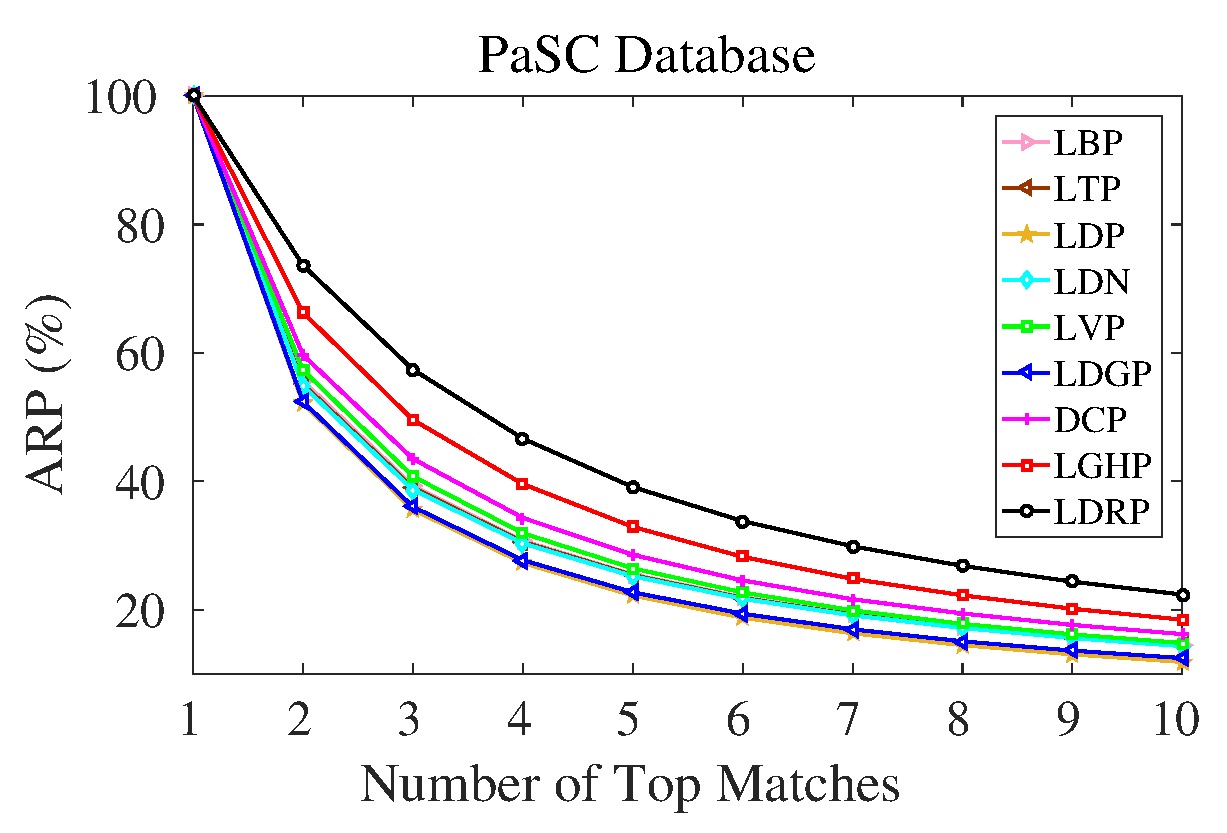
\includegraphics[width=.98\linewidth]{pasc-arp}
    \caption{ARP over PaSC Database}
    \label{fig:pasc-arp}
  \end{subfigure}%
    \begin{subfigure}{.25\textwidth}
    \centering
    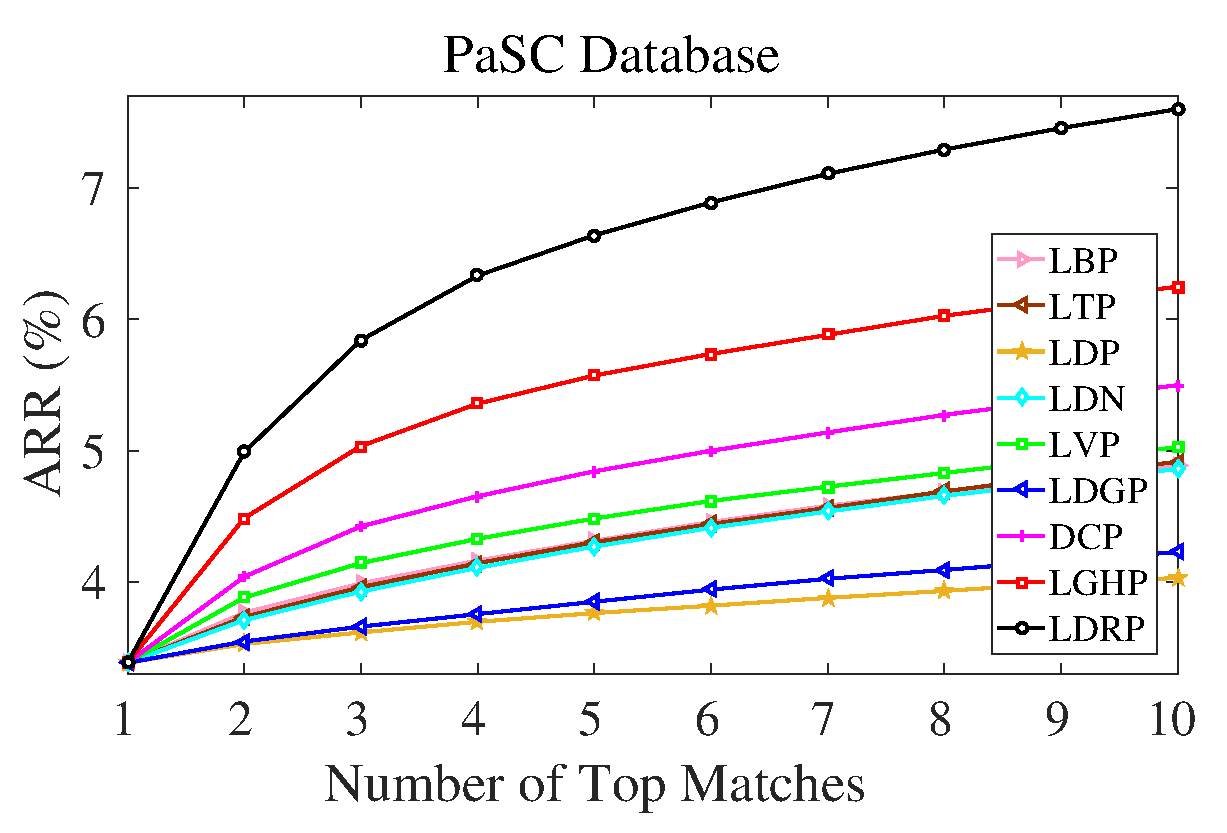
\includegraphics[width=.98\linewidth]{pasc-arr}
    \caption{ARR over PaSC Database}
    \label{fig:pasc-arr}
  \end{subfigure}%
    \begin{subfigure}{.25\textwidth}
    \centering
    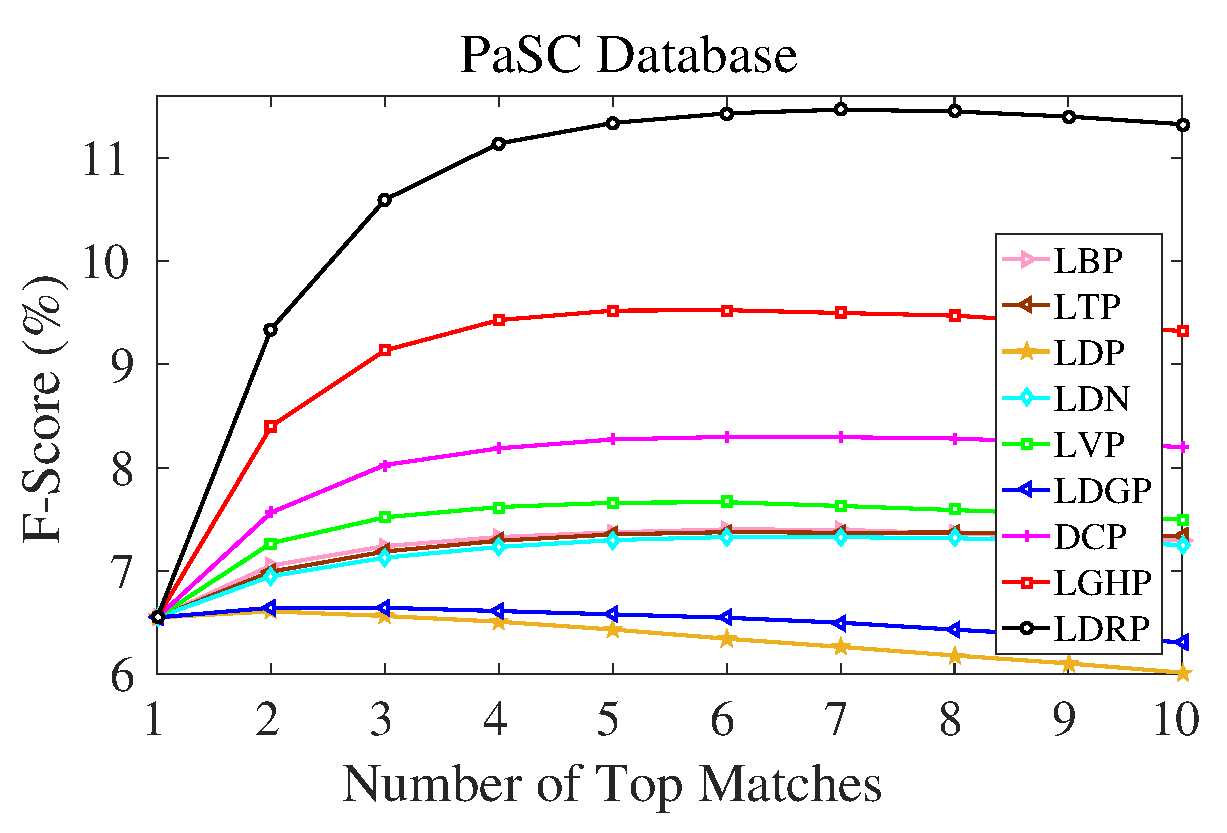
\includegraphics[width=.98\linewidth]{pasc-f}
    \caption{F-Score over PaSC Database}
    \label{fig:pasc-f}
  \end{subfigure}%
    \begin{subfigure}{.25\textwidth}
    \centering
    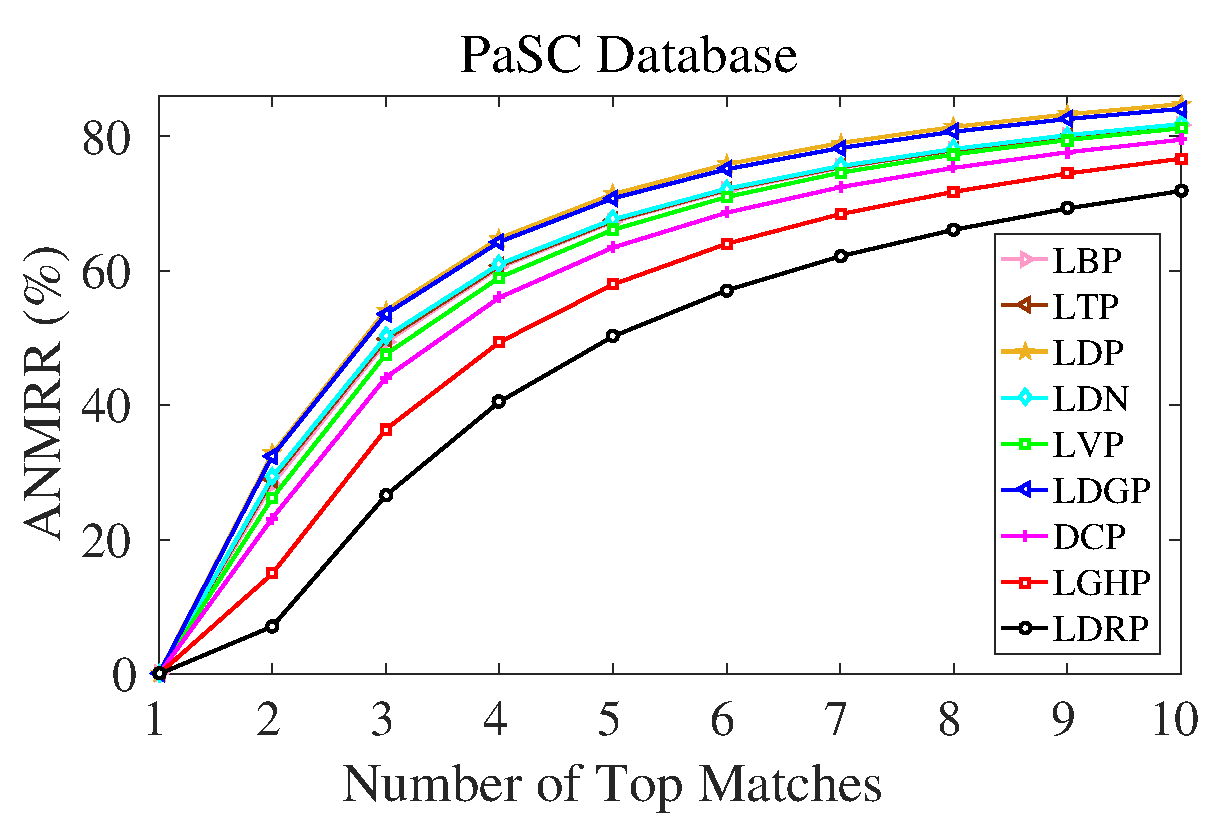
\includegraphics[width=.98\linewidth]{pasc-anmrr}
    \caption{ANMRR over PaSC Database}
    \label{fig:pasc-anmrr}
  \end{subfigure}
  \vspace{3mm}
  
  \begin{subfigure}{.25\textwidth}
    \centering
    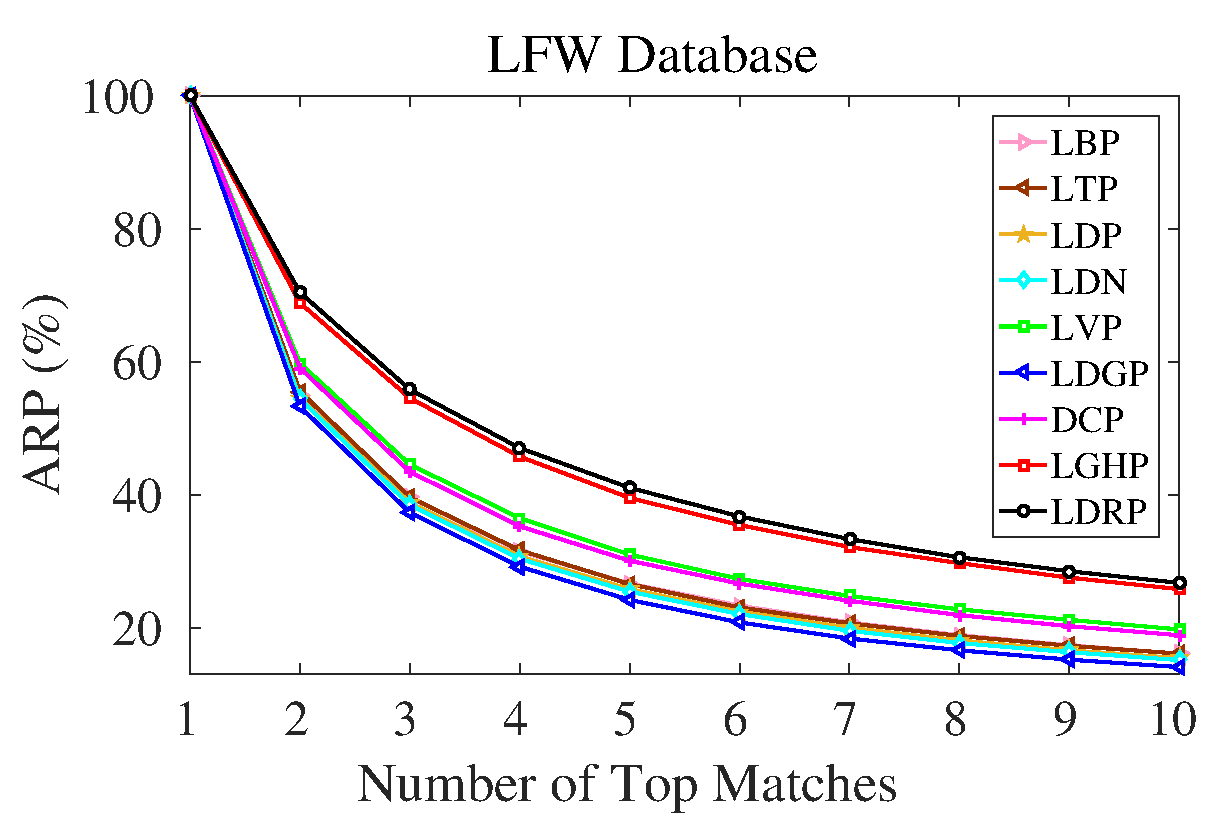
\includegraphics[width=.98\linewidth]{lfw-arp}
    \caption{ARP over LFW Database}
    \label{fig:lfw-arp}
  \end{subfigure}%
    \begin{subfigure}{.25\textwidth}
    \centering
    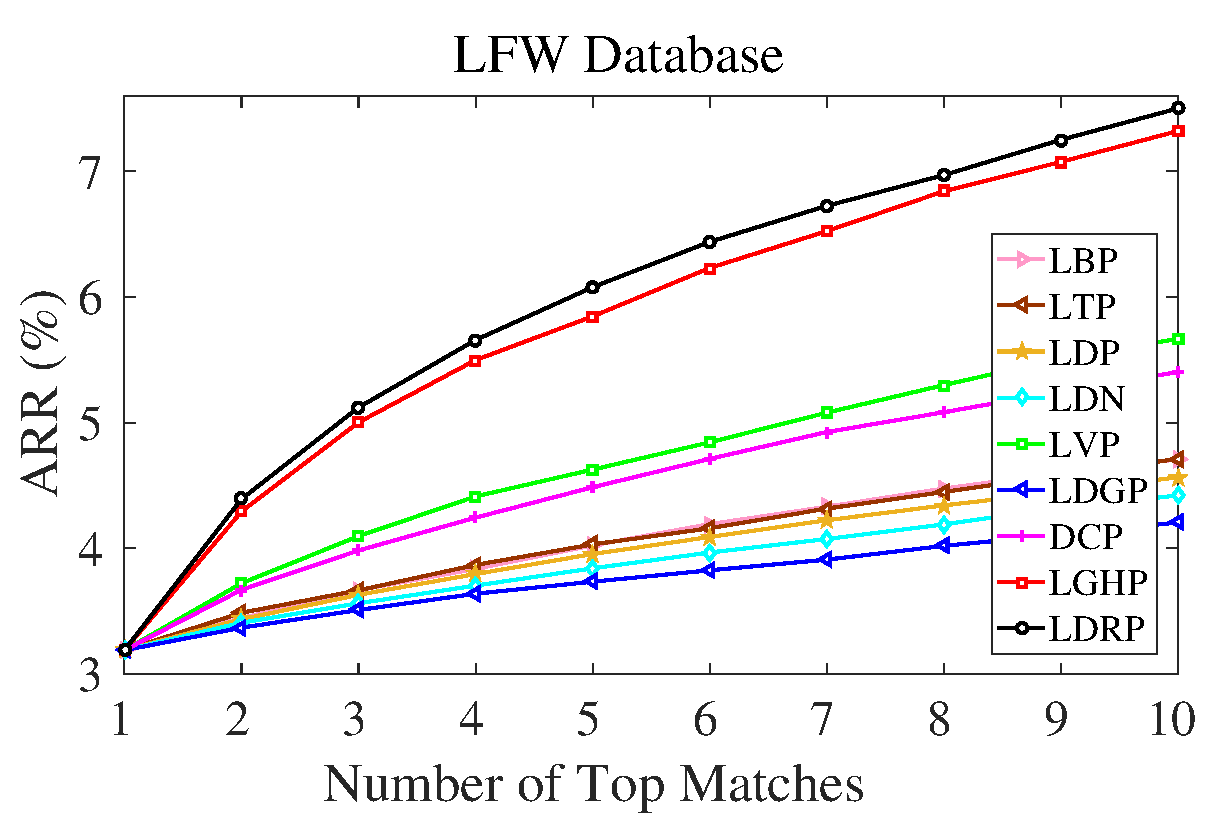
\includegraphics[width=.98\linewidth]{lfw-arr}
    \caption{ARR over LFW Database}
    \label{fig:lfw-arr}
  \end{subfigure}
    \begin{subfigure}{.25\textwidth}
    \centering
    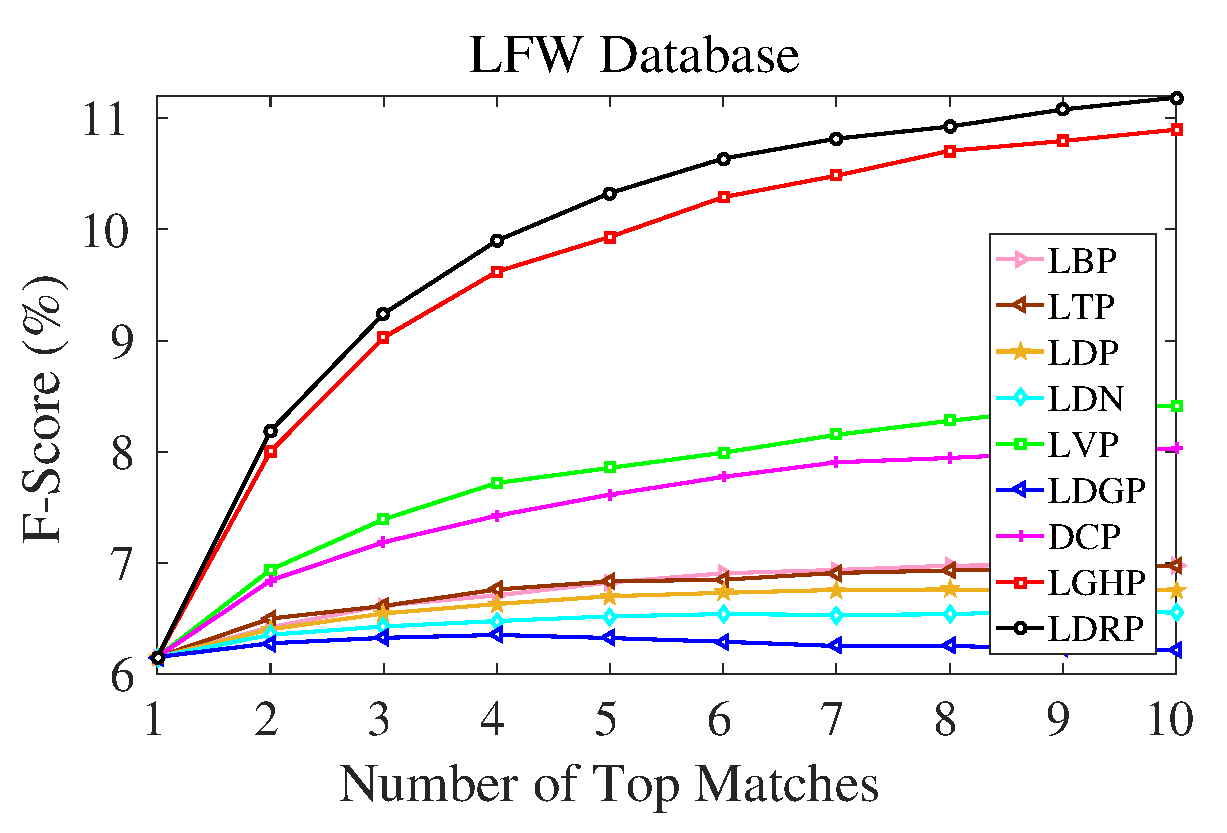
\includegraphics[width=.98\linewidth]{lfw-f}
    \caption{F-Score over LFW Database}
    \label{fig:lfw-f}
  \end{subfigure}%
    \begin{subfigure}{.25\textwidth}
    \centering
    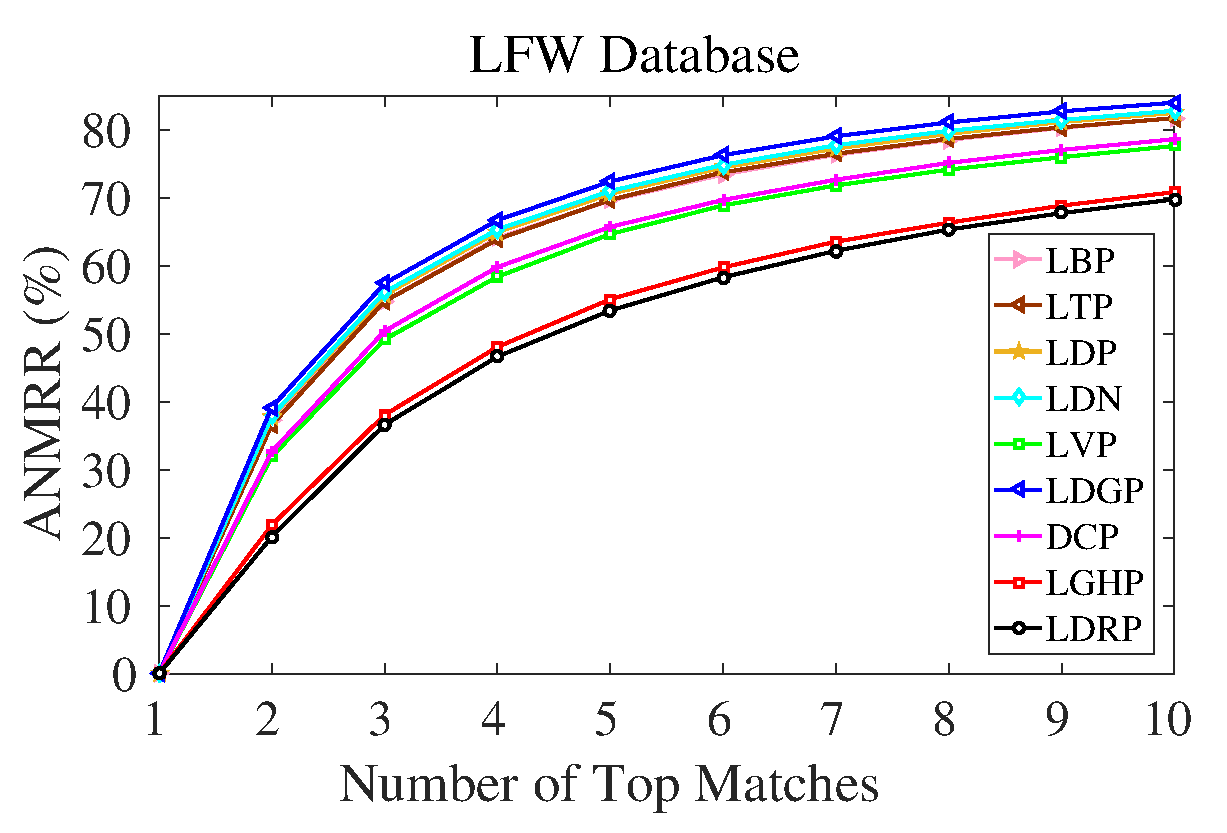
\includegraphics[width=.98\linewidth]{lfw-anmrr}
    \caption{ANMRR over LFW Database}
    \label{fig:lfw-anmrr}
  \end{subfigure}
  \vspace{3mm}
  
  \begin{subfigure}{.25\textwidth}
    \centering
    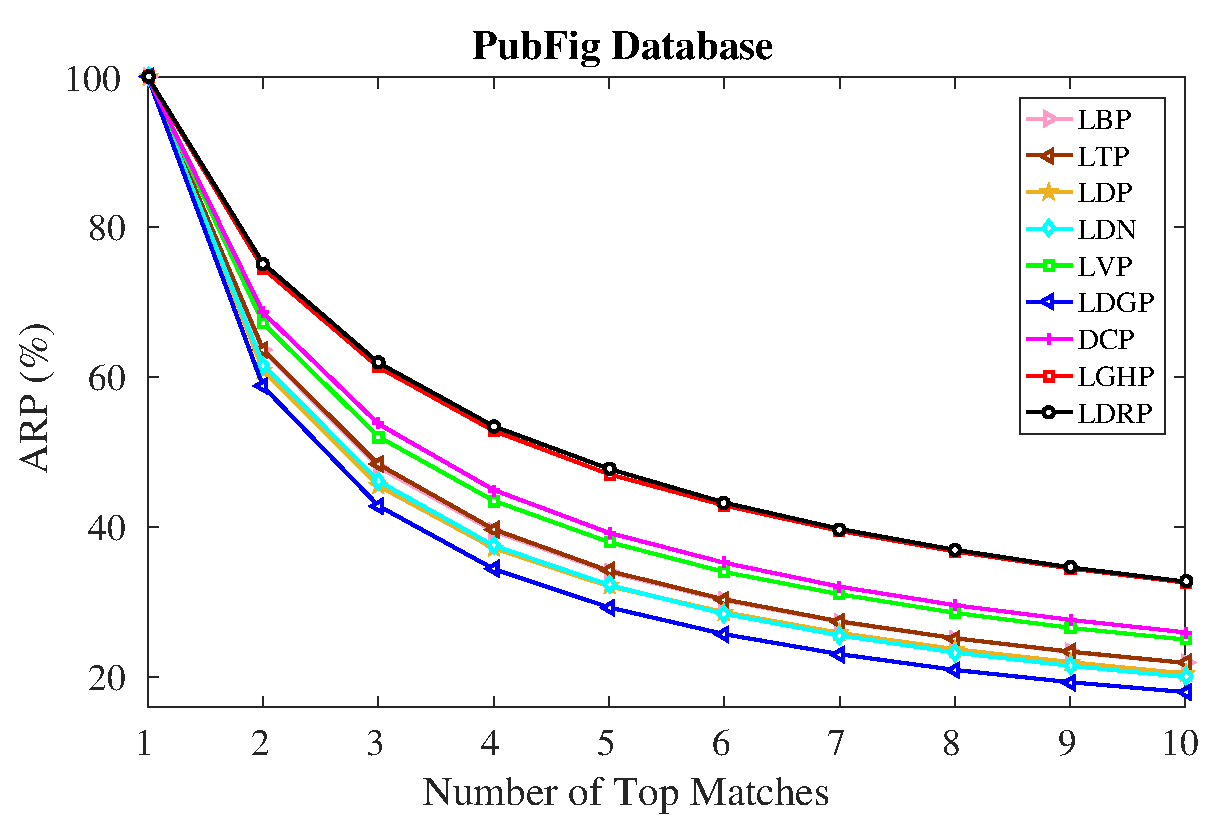
\includegraphics[width=.98\linewidth]{pubfig-arp}
    \caption{ARP over PubFig Database}
    \label{fig:pubfig-arp}
  \end{subfigure}%
    \begin{subfigure}{.25\textwidth}
    \centering
    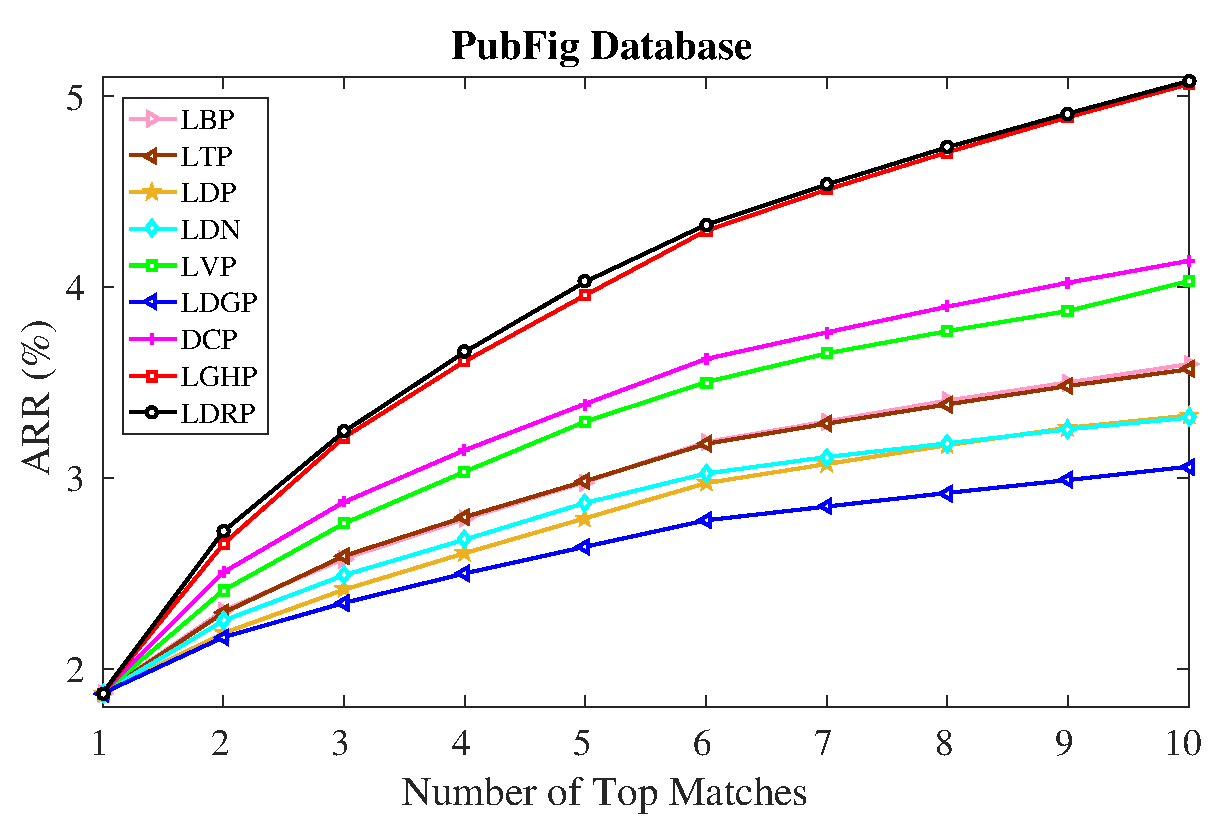
\includegraphics[width=.98\linewidth]{pubfig-arr}
    \caption{ARR over PubFig Database}
    \label{fig:pubfig-arr}
  \end{subfigure}%
    \begin{subfigure}{.25\textwidth}
    \centering
    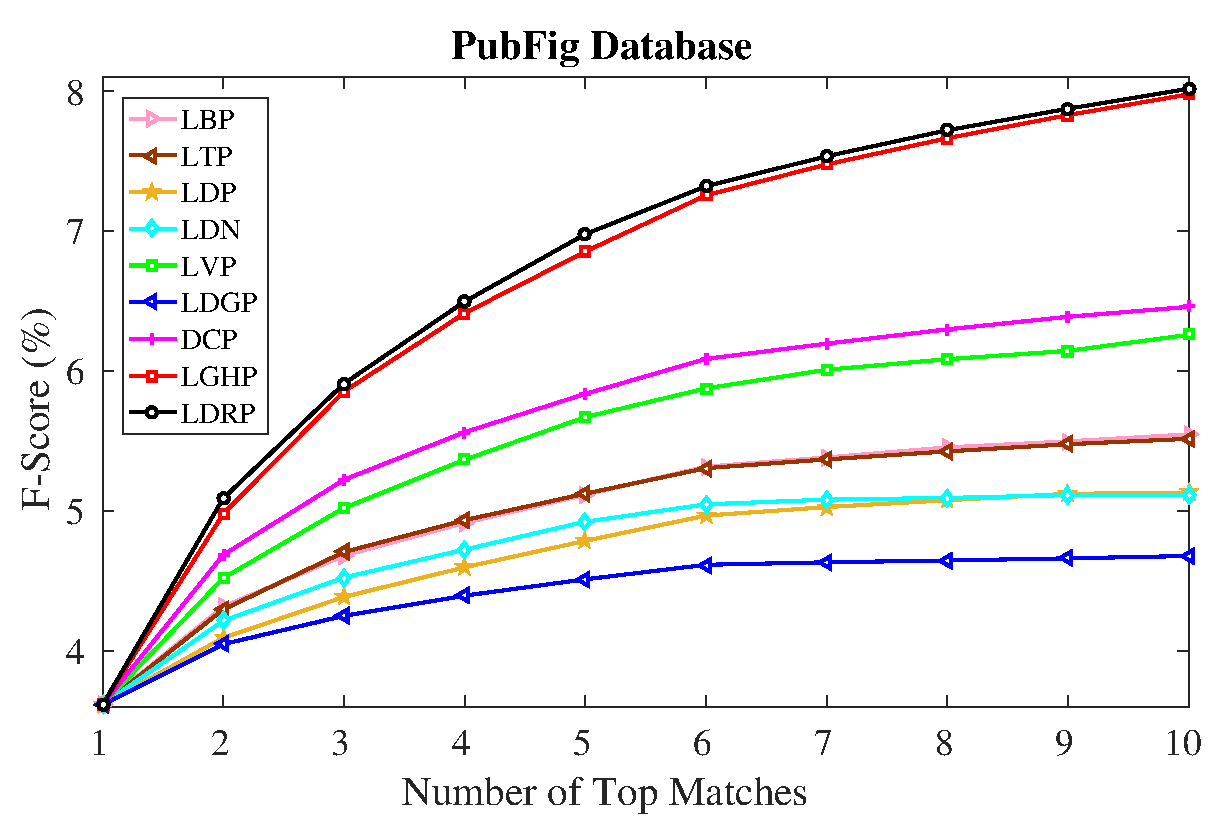
\includegraphics[width=.98\linewidth]{pubfig-f}
    \caption{F-Score over PubFig Database}
    \label{fig:pubfig-f}
  \end{subfigure}%
    \begin{subfigure}{.25\textwidth}
    \centering
    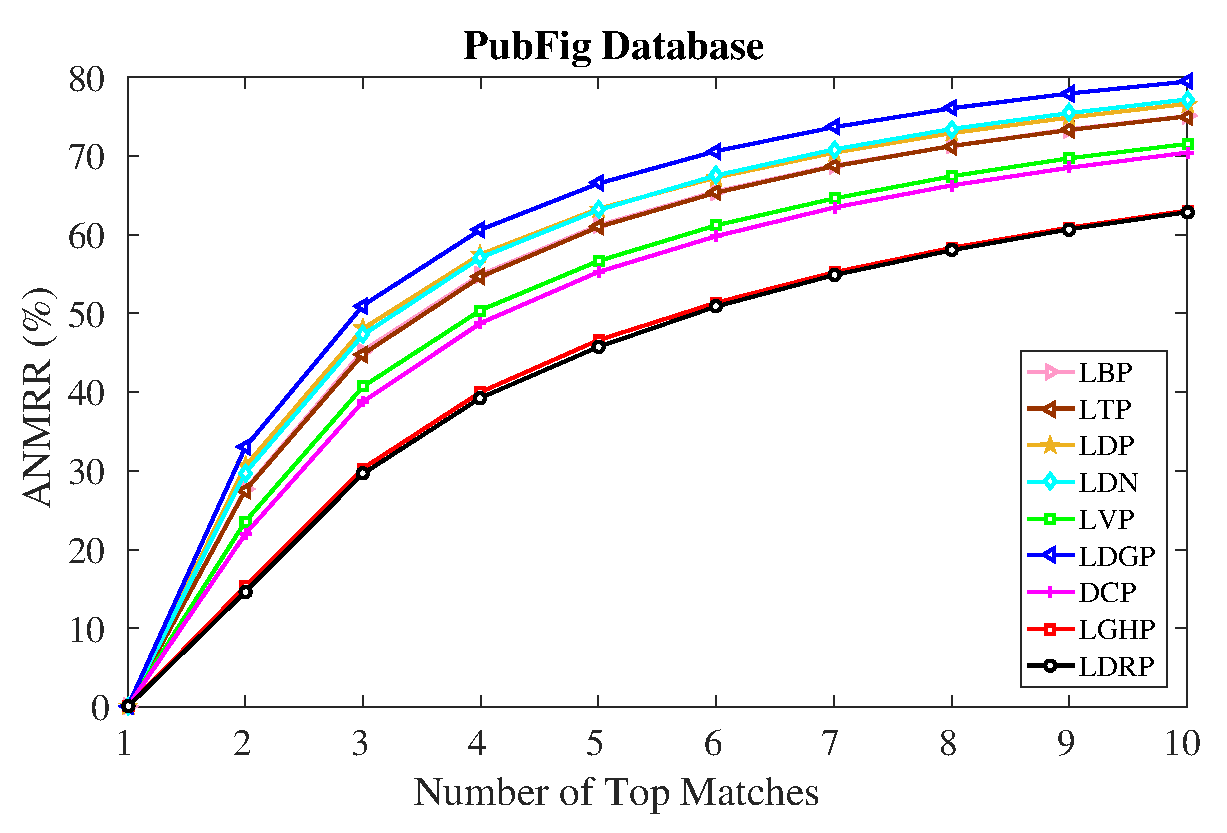
\includegraphics[width=.98\linewidth]{pubfig-anmrr}
    \caption{ANMRR over PubFig Database}
    \label{fig:pubfig-anmrr}
  \end{subfigure}
  \vspace{3mm}
  
  \begin{subfigure}{.25\textwidth}
    \centering
    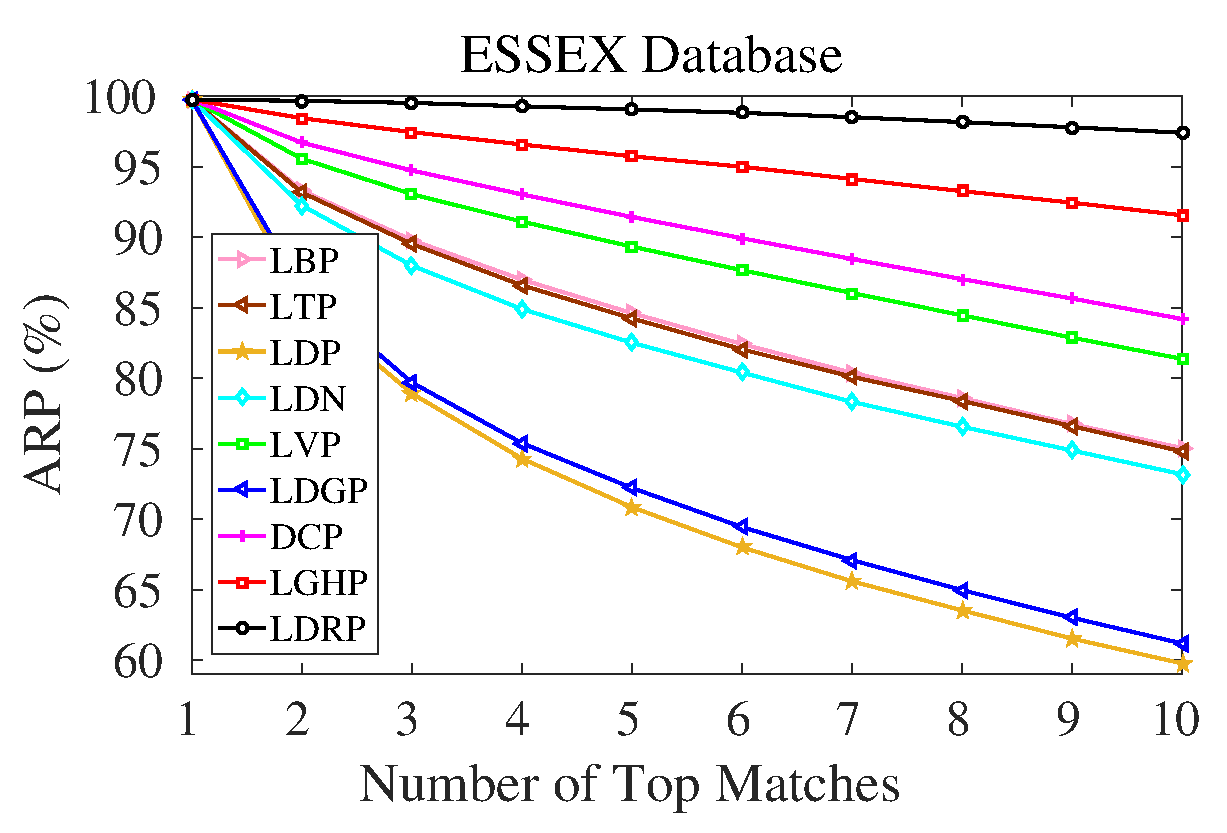
\includegraphics[width=.98\linewidth]{essex-arp}
    \caption{ARP over ESSEX Database}
    \label{fig:essex-arp}
  \end{subfigure}%
    \begin{subfigure}{.25\textwidth}
    \centering
    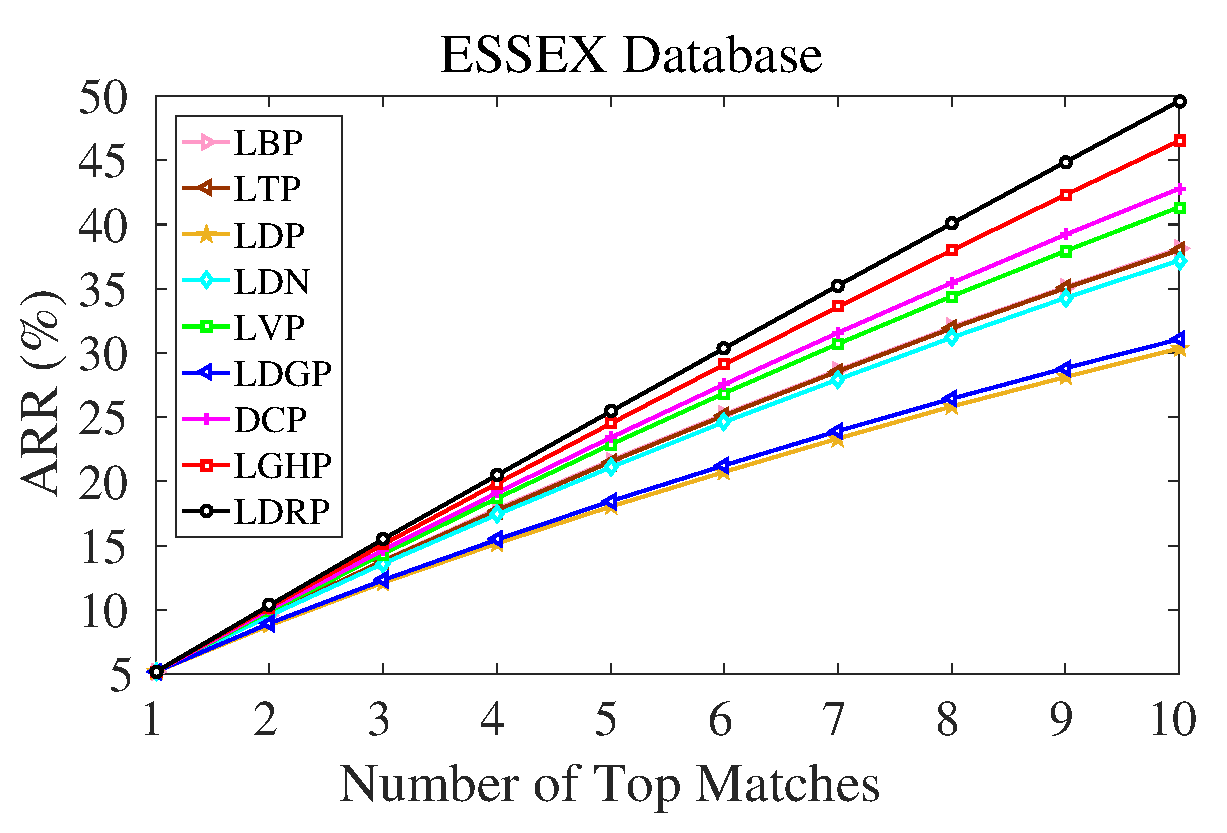
\includegraphics[width=.98\linewidth]{essex-arr}
    \caption{ARR over ESSEX Database}
    \label{fig:essex-arr}
  \end{subfigure}%
    \begin{subfigure}{.25\textwidth}
    \centering
    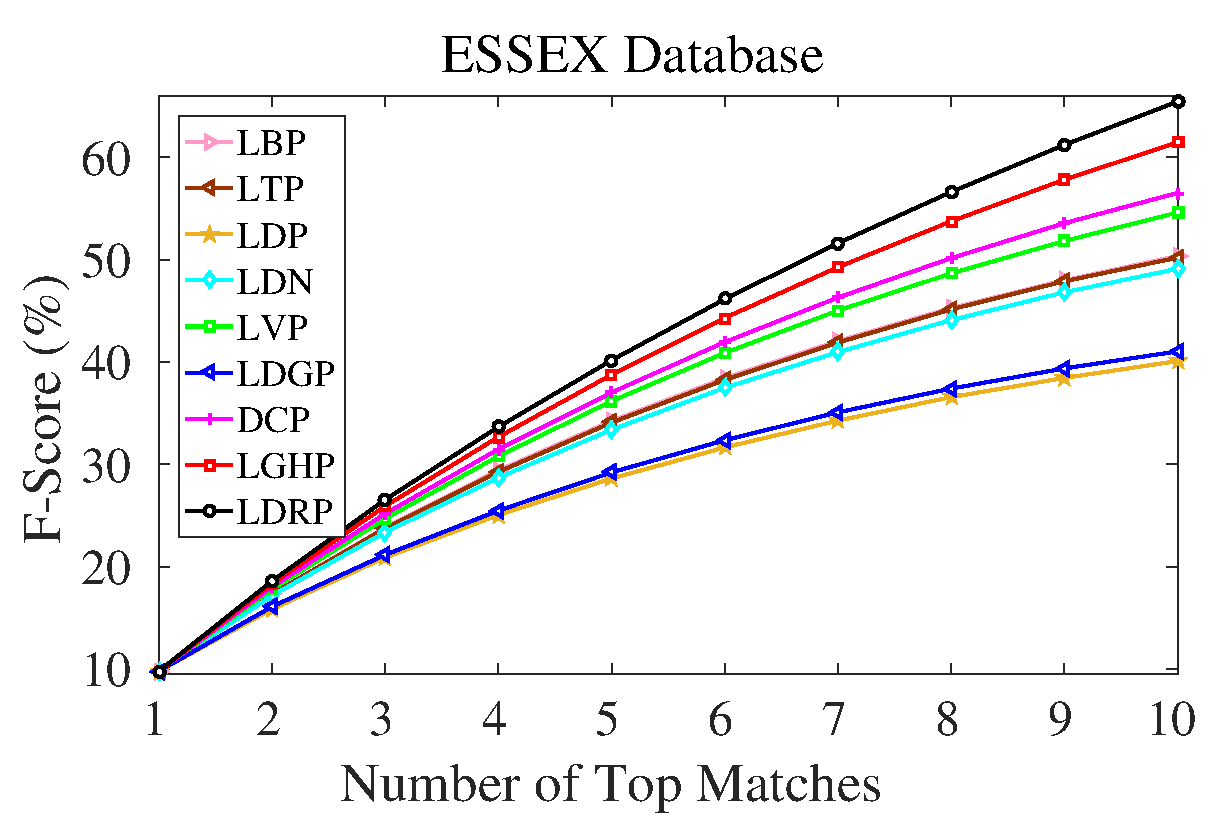
\includegraphics[width=.98\linewidth]{essex-f}
    \caption{F-Score over ESSEX Database}
    \label{fig:essex-f}
  \end{subfigure}%
    \begin{subfigure}{.25\textwidth}
    \centering
    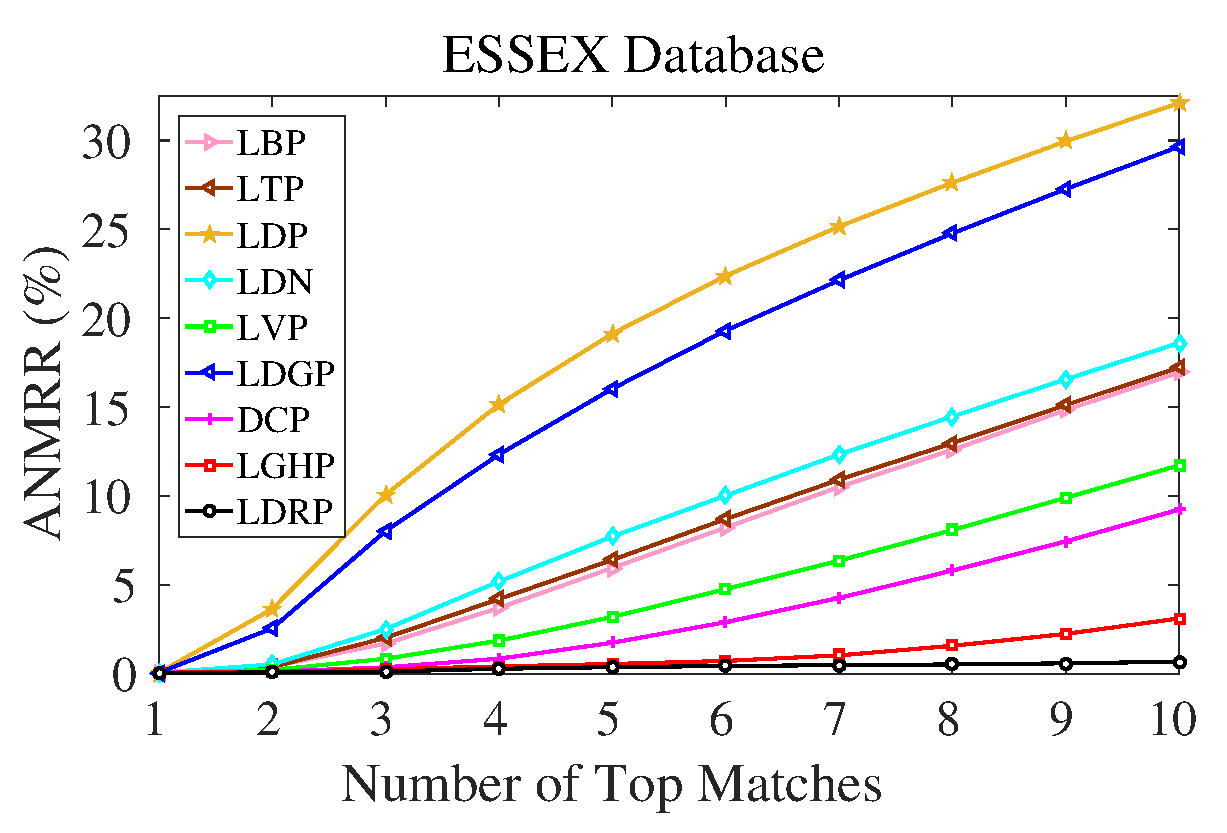
\includegraphics[width=.98\linewidth]{essex-anmrr}
    \caption{ANMRR over ESSEX Database}
    \label{fig:essex-anmrr}
  \end{subfigure}
  \vspace{3mm}
  
  \begin{subfigure}{.25\textwidth}
    \centering
    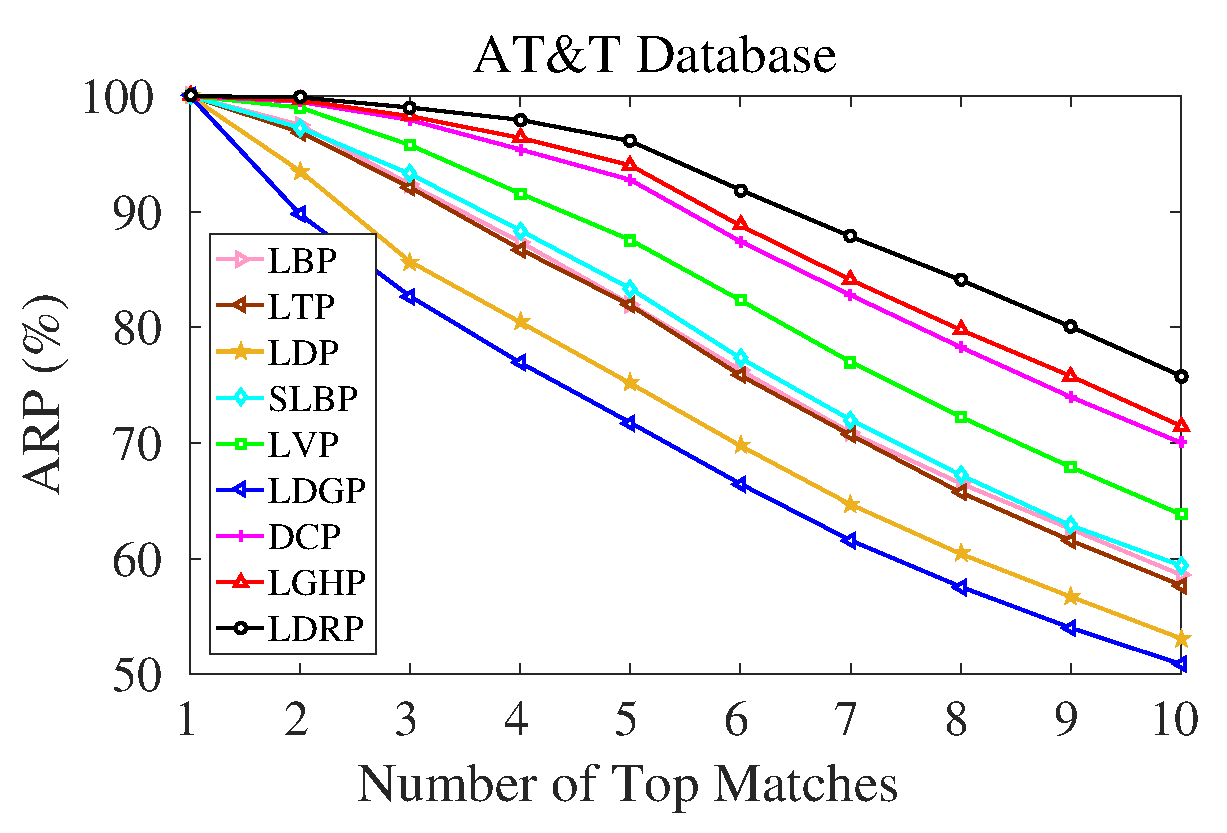
\includegraphics[width=.98\linewidth]{att-arp}
    \caption{ARP over AT\&T Database}
    \label{fig:att-arp}
  \end{subfigure}%
    \begin{subfigure}{.25\textwidth}
    \centering
    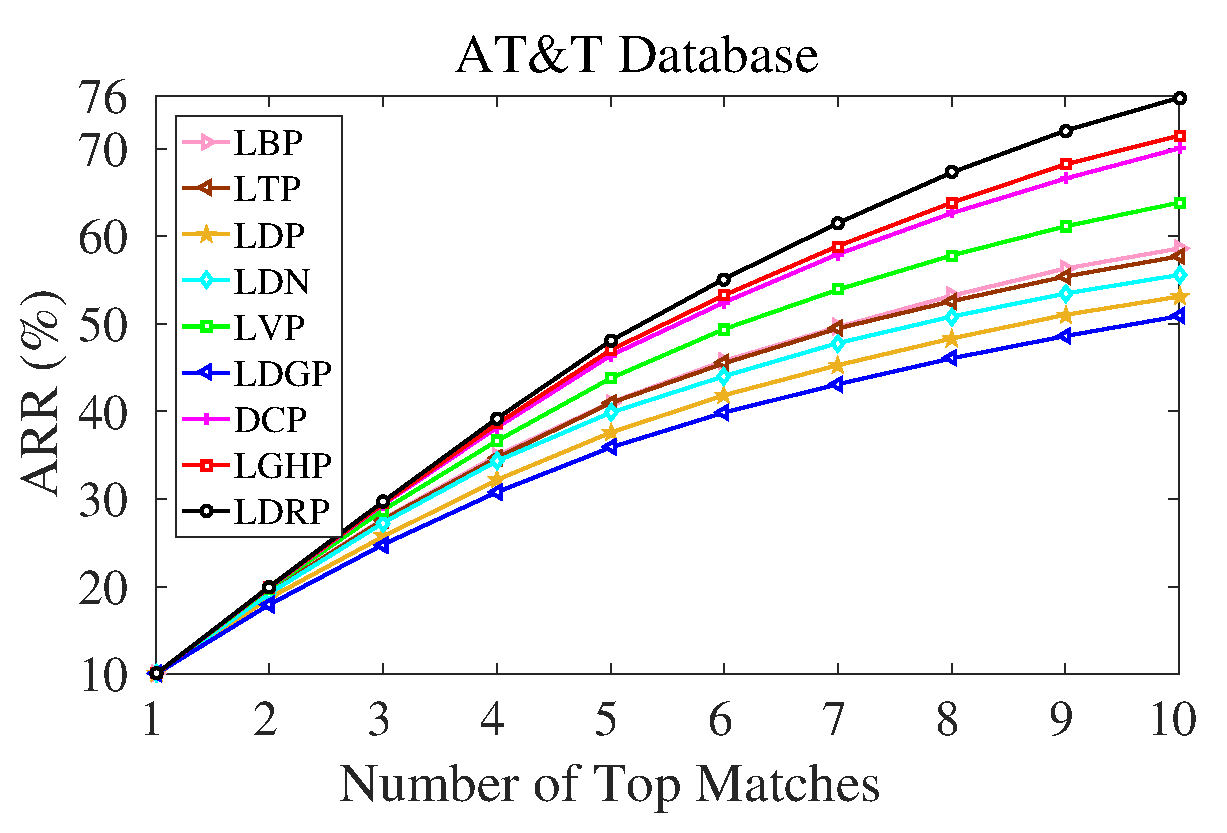
\includegraphics[width=.98\linewidth]{att-arr}
    \caption{ARR over AT\&T Database}
    \label{fig:att-arr}
  \end{subfigure}%
    \begin{subfigure}{.25\textwidth}
    \centering
    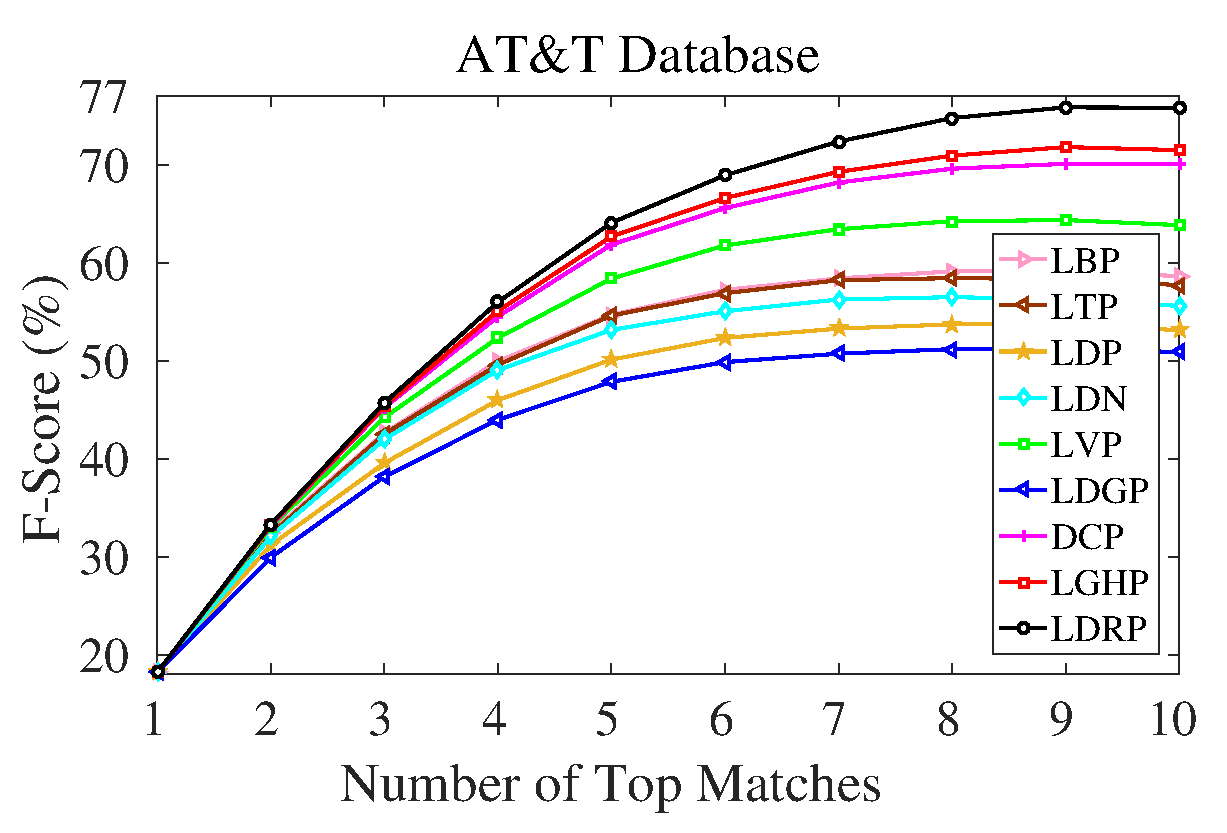
\includegraphics[width=.98\linewidth]{att-f}
    \caption{F-Score over AT\&T Database}
    \label{fig:att-f}
  \end{subfigure}%
    \begin{subfigure}{.25\textwidth}
    \centering
    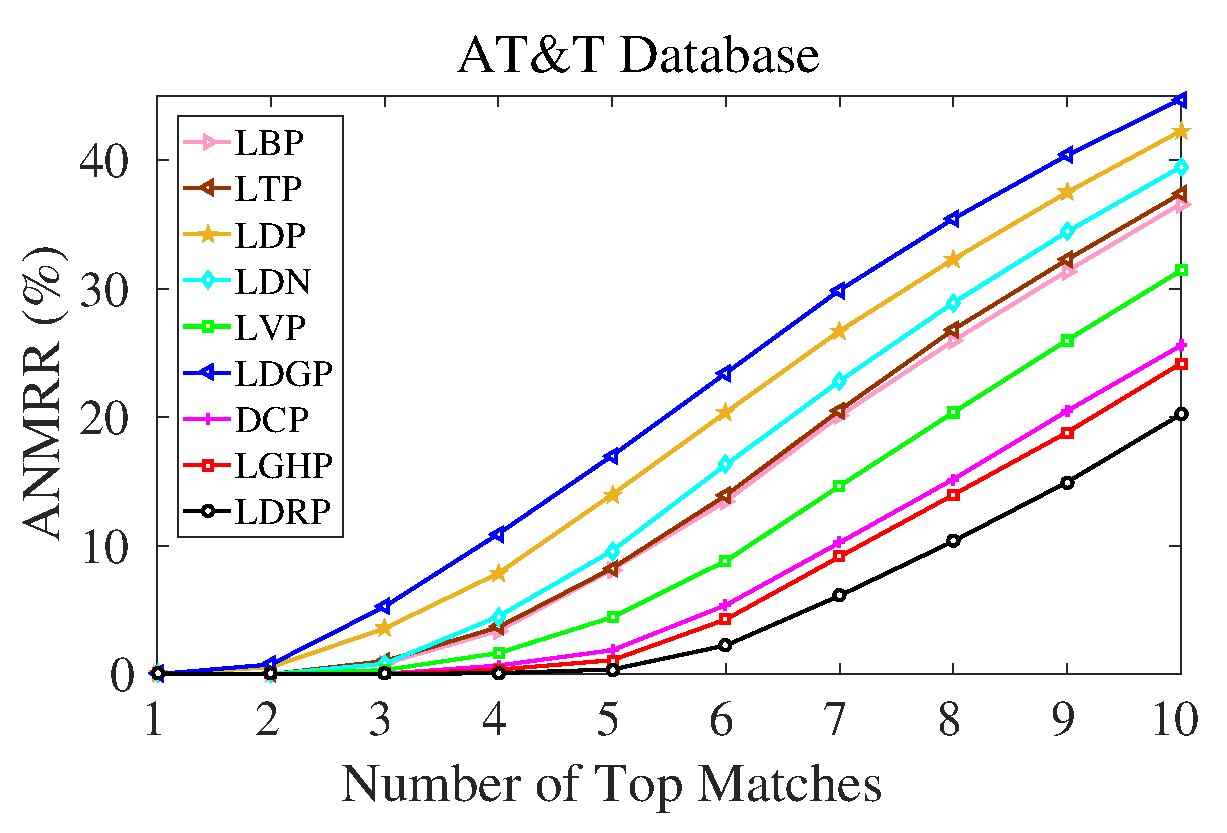
\includegraphics[width=.98\linewidth]{att-anmrr}
    \caption{ANMRR over AT\&T Database}
    \label{fig:att-anmrr}
  \end{subfigure}
  \vspace{3mm}
  
  \begin{subfigure}{.25\textwidth}
    \centering
    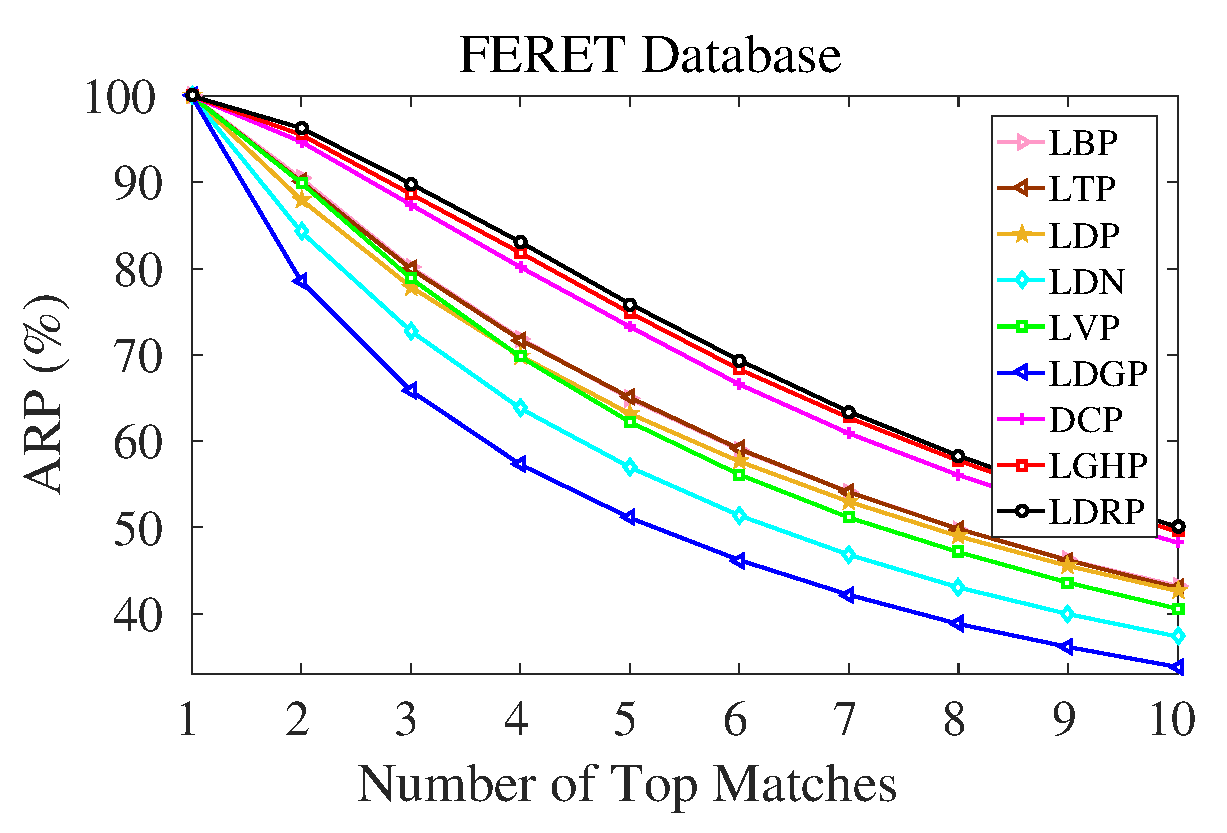
\includegraphics[width=.98\linewidth]{feret-arp}
    \caption{ARP over FERET Database}
    \label{fig:feret-arp}
  \end{subfigure}%
    \begin{subfigure}{.25\textwidth}
    \centering
    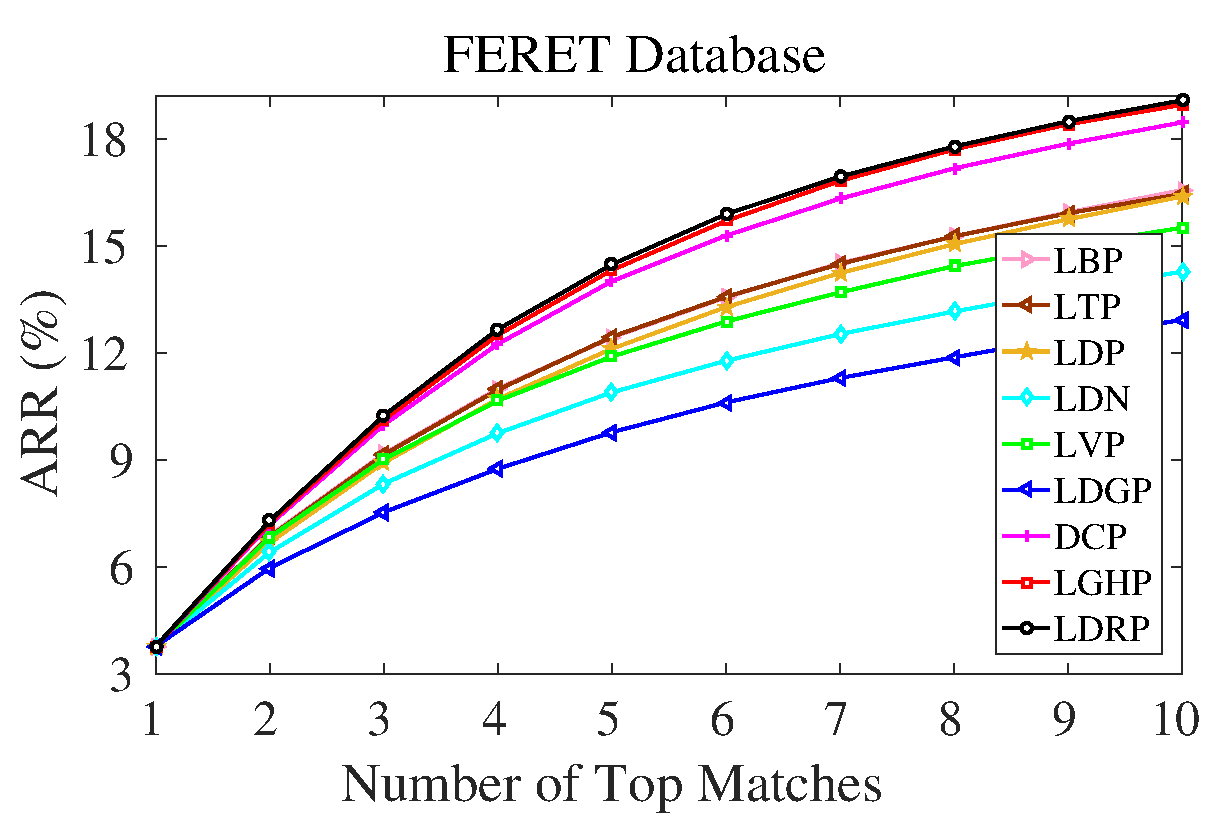
\includegraphics[width=.98\linewidth]{feret-arr}
    \caption{ARR over FERET Database}
    \label{fig:feret-arr}
  \end{subfigure}%
    \begin{subfigure}{.25\textwidth}
    \centering
    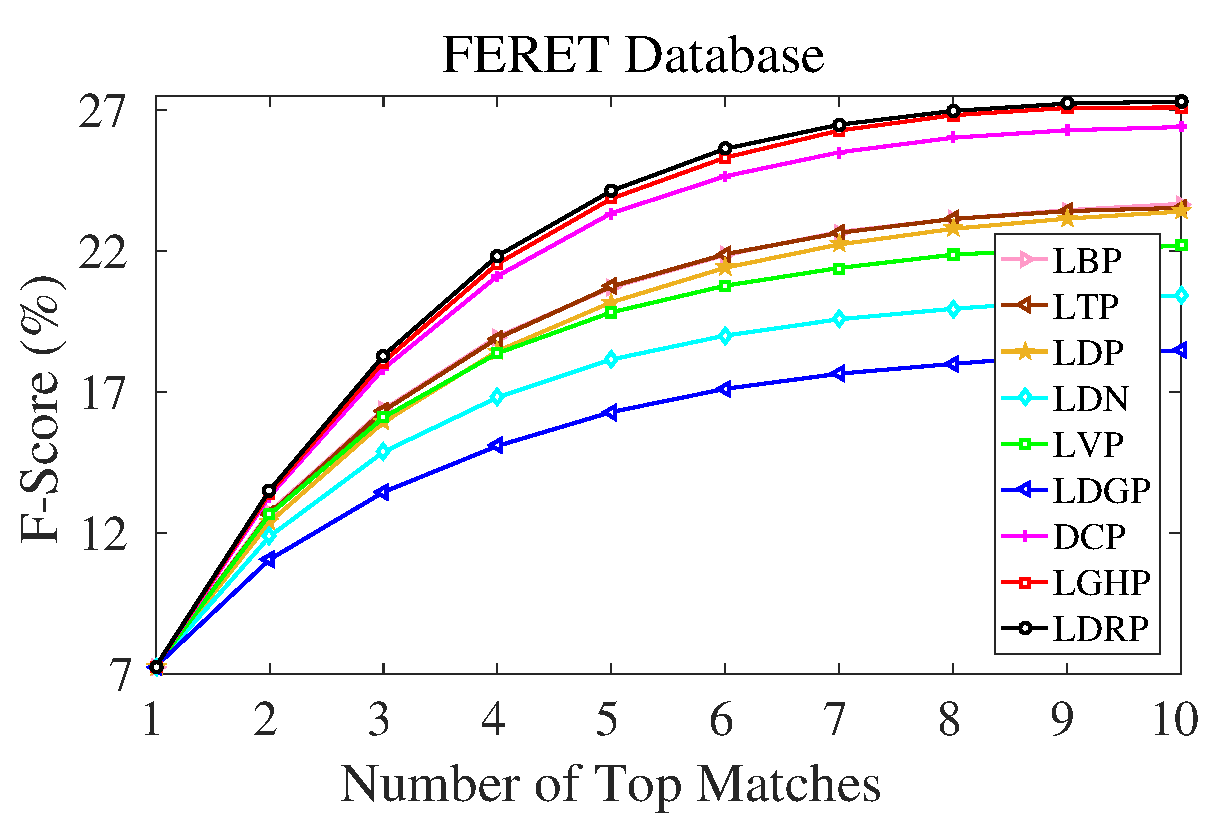
\includegraphics[width=.98\linewidth]{feret-f}
    \caption{F-Score over FERET Database}
    \label{fig:feret-f}
  \end{subfigure}%
    \begin{subfigure}{.25\textwidth}
    \centering
    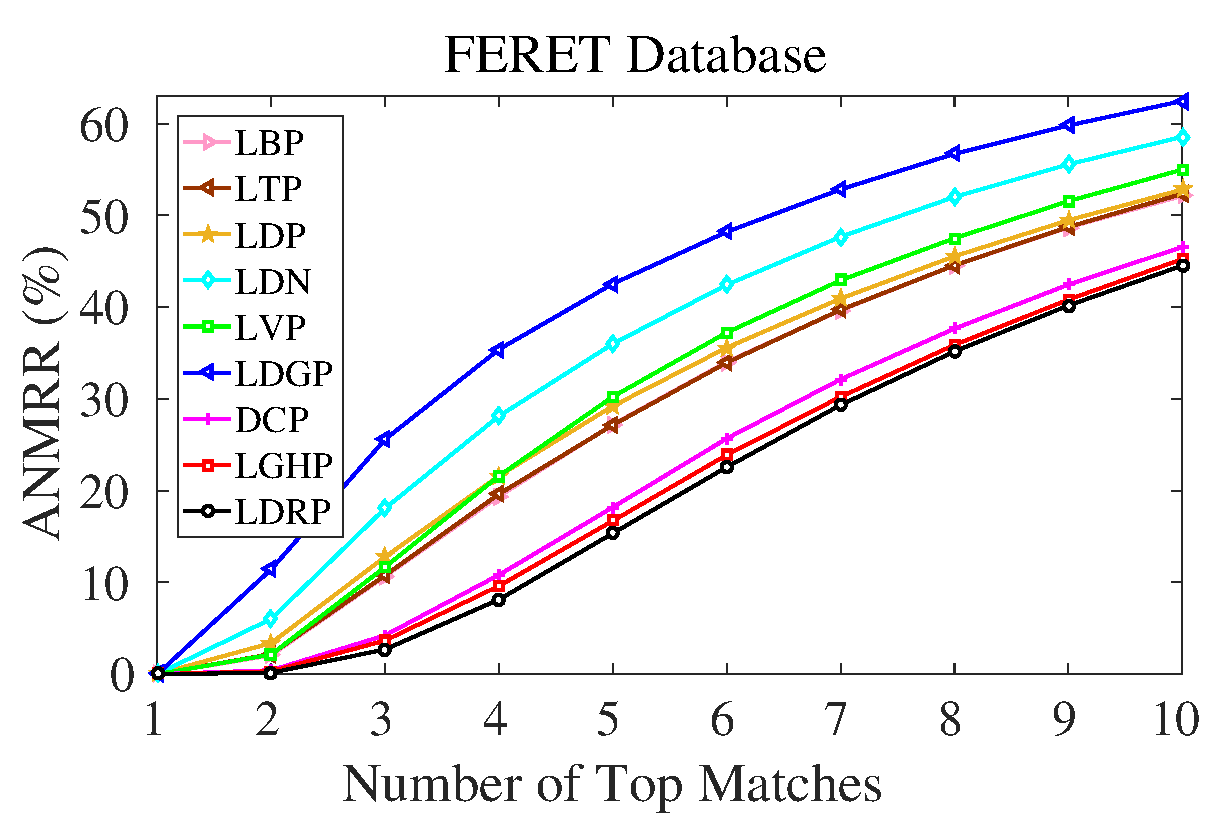
\includegraphics[width=.98\linewidth]{feret-anmrr}
    \caption{ANMRR over FERET Database}
    \label{fig:feret-anmrr}
  \end{subfigure}
  \vspace{2mm}
  
  \caption{The results over PaSC, LFW, PubFig, ESSEX, AT\&T, and FERET databases in terms of the ARP, ARR, F-Score, and ANMRR vs number of retrieved images.}
  \label{fig:results}
\end{figure*}



In order to demonstrate the superior performance of proposed local directional relation pattern (LDRP) descriptor for face retrieval, the state-of-the-art face descriptors like LBP \cite{lbp}, LTP
\cite{ltp}, LDP \cite{ldp}, LDN \cite{ldn}, LVP \cite{lvp}, LDGP \cite{ldgp}, DCP \cite{dcp}, and LGHP \cite{lghp} are used for the comparison over all six databases. The dimensions of LBP, LTP, LDP, LDN, LVP, LDGP, DCP, LGHP, and LDRP descriptors are 256, 512, 1024, 64, 1024, 65, 512, 9216, and 1024 respectively. Note that, all these descriptors have shown very promising results for facial analysis under varying conditions such as rotation, scale, background, blur, illumination, pose, masking, etc. The parameters for all the compared descriptors are  used as per their source papers.

The results comparison using different descriptors in terms of the ARP (\%), ARR (\%), F-score (\%) and ANMRR (\%) vs number of retrieved images ($n$) over PaSC, LFW, PubFig, ESSEX, AT\&T and FERET face databases are presented in Fig. \ref{fig:results}. The $1^{st}$, $2^{nd}$, ${3^{rd}}$, ${4^{th}}$, ${5^{th}}$, and ${6^{th}}$ rows correspond to the results over PaSC, LFW, PubFig, ESSEX, AT\&T and FERET face databases respectively. The $1^{st}$, $2^{nd}$, ${3^{rd}}$, and ${4^{th}}$ columns correspond to ARP(\%) vs $n$, ARR(\%) vs $n$, F-Score(\%) vs $n$, and ANMRR(\%) vs $n$ respectively. 
The LDRP descriptor outperforms the existing face descriptors over PaSC database as it has the highest values for ARP, ARR, and F-Score and lowest values for ANMRR (see Fig. \ref{fig:pasc-arp}-\ref{fig:pasc-anmrr}). PaSC database is having variations like scale, blur, pose and illumination. The LFW and PubFig databases are fully unconstrained database. It is observed that the performance of LDRP descriptor is comparable with the LGHP descriptor over both LFW and PubFig databases as depicted in Fig. \ref{fig:lfw-arp}-\ref{fig:lfw-anmrr} and Fig. \ref{fig:pubfig-arp}-\ref{fig:pubfig-anmrr} respectively, whereas the dimension of LDRP(dim: 1024) is much lower than the dimension of LGHP(dim: 9216). Thus, the time efficiency of LDRP is far better than LGHP while maintaining similar performance over the unconstrained databases. 

The performance of LDRP is improved significantly over the frontal face databases, but with other variations like scale, background, illumination, blur, expressions, etc. as shown in Fig. \ref{fig:essex-arp}-\ref{fig:essex-anmrr} over ESSEX database and Fig. \ref{fig:att-arp}-\ref{fig:att-anmrr} over AT\&T database. The proposed LDRP descriptor is outstanding over both ESSEX and AT\&T databases as compared to the state-of-the-art face descriptors. In order to test the suitability of LDRP in pose and scale variations, FERET database is considered because it has the faces with huge pose and scale variations. The results over FERET database is summarized in Fig. \ref{fig:feret-arp}-\ref{fig:feret-anmrr}. It is found that the LDRP is equivalent to the other top performing descriptors such as LGHP over FERET database, whereas its dimension is much lower than LGHP. 

From the experimental results of Fig. \ref{fig:results}, it is observed that LDRP and LGHP descriptors outperforms the other descriptors over the PaSC, LFW, PubFig, ESSEX, AT\&T, and FERET face databases. It is also noticed that the LGHP descriptor is mostly the second best performing method and having very good discriminative features, but redundant and at the cost of increased dimensionality. Whereas, it is clear from Fig. \ref{fig:results} results that despite of having much lower dimensionality, the proposed LDRP descriptor is either outperforms LGHP or has the comparable performance against LGHP. 

\begin{table}[!t]
\caption{The performance comparison of LDRP descriptors in terms of the ARP(\%) for $n=5$ number of retrieved images over the PubFig, PaSC, LFW, FERET, AT\&T, and ESSEX face databases by varying the values of $M_1$ and $M_2$ (i.e. multiscale parameters) for different radius and the number of local neighborhoods. The Chi-square distance is used. The highest ARP values are highlighted in bold for each database.}
\label{t1}
\begin{center}
\begin{tabular}{cccccccc}
\hline
\\[-0.65em] \multirow{2}{*}{$M_1$} & \multirow{2}{*}{$M_1$} & \multicolumn{6}{c}{Face Databases}\\ \\[-0.65em]
\cline{3-8} 
\\[-0.65em]  & & PubFig & PaSC & LFW & FERET & AT\&T & ESSEX \\ \\[-0.65em]
\hline
\\[-0.65em]
3 & 3 & 39.90 & 26.25 & 32.18 & 67.51 & 89.80 & 82.78\\ \\[-0.85em]
3 & 4 & 43.81 & 33.43 & 37.07 & 74.44 & 94.95 & 98.34\\ \\[-0.85em]
3 & 5 & 45.83 & 36.92 & 39.36 & 75.62 & 95.35 & 98.88\\ \\[-0.85em]
3 & 6 & 47.76 & 39.12 & 41.04 & \textbf{75.91} & 96.10 & 99.05\\ \\[-0.85em]
3 & 7 & 48.61 & 40.96 & 42.15 & 75.90 & \textbf{96.30} & 99.11\\ \\[-0.85em]
4 & 4 & 43.24 & 38.28 & 38.42 & 70.61 & 94.50 & 98.44\\ \\[-0.85em]
4 & 5 & 46.53 & 42.09 & 41.00 & 73.47 & 94.45 & 99.01\\ \\[-0.85em]
4 & 6 & 48.08 & 44.20 & 42.75 & 74.07 & 95.65 & 99.07\\ \\[-0.85em]
4 & 7 & \textbf{49.22} & 45.74 & \textbf{44.05} & 74.07 & 96.05 & \textbf{99.14}\\ \\[-0.85em]
5 & 5 & 44.17 & 42.99 & 37.26 & 69.12 & 92.65 & 98.91\\ \\[-0.85em]
5 & 6 & 46.50 & 45.42 & 40.47 & 71.21 & 94.35 & 99.05\\ \\[-0.85em]
5 & 7 & 48.01 & \textbf{46.86} & 42.51 & 71.87 & 95.30 & 99.10\\ \\[-0.85em]
6 & 6 & 44.20 & 43.86 & 37.55 & 67.86 & 93.55 & 98.87\\ \\[-0.85em]
6 & 7 & 46.32 & 45.97 & 40.47 & 69.86 & 95.10 & 99.03\\ \\[-0.85em]
7 & 7 & 43.66 & 44.08 & 37.58 & 66.71 & 93.70 & 98.86\\ \\[-0.65em]
\hline
\end{tabular}
\end{center}
\end{table}


\section{Performance Analysis}
This section is devoted to the performance analysis of the proposed descriptor. First, the effect of size of local neighborhood and multi-scale is analyzed, and then the effect of distance measure is tested over each database. 

\subsection{Effect of Local Neighborhood}
In the previous experiment, the LDRP parameters are as follows: $N=8$, $M_1=3$, and $M_2=6$. In this subsection, the performance of LDRP is tested by varying the values of $M_1$ and $M_2$ from 3 to 7. The ARP(\%) values for $n=5$ number of retrieved images over the PubFig, PaSC, LFW, FERET, AT\&T, and ESSEX face databases are summarized in Table \ref{t1}. The highest ARP for a particular database is highlighted in bold. It is observed that LDRP with $M_1=3$ and $M_2=6$ is having highest precision only over the FERET database. It is due to the huge pose variations present in the FERET database. The performance of LDRP is improved over each database for upper limit as a maximum (i.e. $M_2=7$). From this experiment, it is also clear that $M_1=4$ and $M_2=7$ are better suited for unconstrained scenario. Though, $M_1=3$ and $M_2=6$ are used in the previous results, the performance of LDRP can be further improved by considering $M_1=4$ and $M_2=7$.


\subsection{Effect of Distance Measures}

\begin{table}[!t]
\caption{The ARP(\%) using proposed LDRP descriptor with Euclidean, Cosine, L1, D1, and Chi-square distance measures over the PubFig, PaSC, LFW, FERET, AT\&T, and ESSEX face databases. The number of retrieved images ($n$) is 5. The highest ARP values are highlighted in bold for each database.}
\label{t2}
\begin{center}
\begin{tabular}{lcccccc}
\hline
\\[-0.65em]\multirow{2}{*}{Distance} & \multicolumn{6}{c}{Face Databases}\\ \\[-0.65em]
\cline{2-7} 
\\[-0.65em] & PubFig & PaSC & LFW & FERET & AT\&T & ESSEX \\ \\[-0.65em]
\hline
\\[-0.65em]
Euclidean & 35.49 & 27.53 & 30.17 & 65.09 & 88.45 & 95.83\\ \\[-0.85em]
Cosine & 37.24 & 30.93 & 32.37 & 67.23 & 93.40 & 97.46\\ \\[-0.85em]
L1 & 44.91 & 36.96 & 38.57 & 75.54 & 95.50 & 98.80\\ \\[-0.85em]
D1 & 45.25 & 37.62 & 39.14 & 75.53 & 95.65 & 98.86\\ \\[-0.85em]
Chi-square & \textbf{47.76} & \textbf{39.12} & \textbf{41.04} & \textbf{75.91} & \textbf{96.10} & \textbf{99.05}\\ \\[-0.65em]
\hline
\end{tabular}
\end{center}
\end{table}


\begin{table}[!t]
\caption{The ARP(\%) using LGHP descriptor \cite{lghp} with Euclidean, Cosine, L1, D1, and Chi-square distance measures over the PubFig, PaSC, LFW, FERET, AT\&T, and ESSEX face databases. The number of retrieved images ($n$) is 5. The highest ARP values are highlighted in bold for each database.}
\label{t3}
\begin{center}
\begin{tabular}{lcccccc}
\hline
\\[-0.65em]\multirow{2}{*}{Distance} & \multicolumn{6}{c}{Face Databases}\\ \\[-0.65em]
\cline{2-7} 
\\[-0.65em] & PubFig & PaSC & LFW & FERET & AT\&T & ESSEX \\ \\[-0.65em]
\hline
\\[-0.65em]
Euclidean & 34.28 & 24.21 & 27.82 & 49.11 & 81.90 & 90.57\\ \\[-0.85em]
Cosine & 36.10 & 25.82 & 29.51 & 54.60 & 83.10 & 91.75\\ \\[-0.85em]
L1 & 43.89 & 30.25 & 36.30 & 69.60 & 91.65 & 95.09\\ \\[-0.85em]
D1 & 43.96 & 30.29 & 36.33 & 69.71 & 91.75 & 95.11\\ \\[-0.85em]
Chi-square & \textbf{47.05} & \textbf{32.93} & \textbf{39.53} & \textbf{74.88} & \textbf{94.00} & \textbf{95.73}\\ \\[-0.65em]
\hline
\end{tabular}
\end{center}
\end{table}

In order to find out the suitable distance measure for the proposed descriptor, this experiment is conducted by using the different distance measures. The Euclidean, Cosine, L1, D1, and Chi-square distances are used in this experiment \cite{ltrp}, \cite{mdlbp}. The ARP in percentage over the PubFig, PaSC, LFW, FERET, AT\&T, and ESSEX databases for $n=5$ number of top matches are displayed in Table \ref{t2} using the proposed LDRP descriptor. In this experiment, the default parameter values are used for LDRP descriptor (i.e., $N=8$, $M_1=3$, and $M_2=6$). The best result over a database is highlighted in bold. It is observed from the results that the Chi-square distance measure is better suited with the proposed LDRP descriptor for a face retrieval task. The effect of distances is also tested with LGHP descriptor \cite{lghp} in Table \ref{t3} and interestingly, the Chi-square distance is also better suited for LGHP. The Chi-square distance is performing better because the descriptors are in the form of histograms and representing the occurrences of patterns in some form.


\section{Conclusion}
In this paper, a local directional relation pattern (LDRP) is proposed that utilizes the wider neighborhood information to increase the discriminative ability and local relations to increase the robustness. The LDRP first converts the wider local neighborhood into local directional codes in order to decrease the dimension of the descriptor by exploiting the relation among the directional neighbors at multiple radius, then it transforms the center pixel into the range of local directional relation codes, and finally the descriptor is computed by utilizing the relation of transformed center pixel with directional relation codes. The proposed LDRP descriptor is tested in an image retrieval framework over six very challenging face databases such as PaSC, LFW, FERET, etc. Some databases are totally unconstrained while some are having very severe variations in pose, expressions, etc. The retrieval results of LDRP are compared with the state-of-the-art face descriptors like LBP, LDN, DCP, LGHP, etc. The experimental results confirm the superiority of the LDRP descriptor as compared to the existing face descriptors. It is noticed that the performance of LDRP can be further boosted by considering more wider neighborhoods. The Chi-square distance measure is found to be best suited with LDRP for face retrieval. 






% use section* for acknowledgment
%\section*{Acknowledgment}
%The authors would like to thank...

% Can use something like this to put references on a page
% by themselves when using endfloat and the captionsoff option.
%\ifCLASSOPTIONcaptionsoff
%  \newpage
%\fi

% references section
\bibliographystyle{IEEEtran}
\bibliography{r1}


\iffalse\begin{IEEEbiography}[{\includegraphics[width=1in,height=1.25in,clip,keepaspectratio]{srd.jpg}}]{Shiv Ram Dubey}
has been with the Indian Institute of Information Technology, Sricity (IIIT Sricity) since June 2016,  where he is currently the Assistant Professor of Computer Science and Engineering.  

He received the Ph.D. degree in Computer Vision and Image Processing from Indian Institute of Information Technology, Allahabad (IIIT Allahabad) in 2016. Before that, from August 2012-Feb 2013, he was a Project Officer in the Computer Science and Engineering Department at Indian Institute of Technology, Madras (IIT Madras).  
He was a recipient of several awards including the Early Career Research Award from SERB, Govt. of India and NVIDIA GPU Grant from NVIDIA. He received Certificate of Reviewing Awards from Biosystems Engineering and Computers in Biology and Medicine, Elsevier in 2015 and 2016 respectively. He received the Best Paper Award in IEEE UPCON 2015, a prestigious conference of IEEE UP Section. 
His research interest includes  Computer Vision, Deep Learning, Image Processing,  Image Feature Description, Image Matching, Content Based Image Retrieval,  Medical Image Analysis  and Biometrics.  
\end{IEEEbiography}\fi



\end{document}


